\documentclass[11pt,compress,t,notes=noshow, aspectratio=169, xcolor=table]{beamer}
\usepackage{../../style/lmu-lecture}
% Defines macros and environments
\input{../../style/common.tex}

\usepackage{multicol}

\newcommand{\Dtestm}{\mathcal{D}_{\text{test}, m}}
% lowr case c vector used only here, was undefined, not in latex-math
\newcommand{\cv}{\mathbf{c}}
\title{Applied Machine Learning}
% \author{LMU}
%\institute{\href{https://compstat-lmu.github.io/lecture_iml/}{compstat-lmu.github.io/lecture\_iml}}
\date{}

\begin{document}


\newcommand{\titlefigure}{figure/imbalanced_data_plot_title}
\newcommand{\learninggoals}{
  \item Know what an imbalanced data set is
  \item Understand disadvantage of accuracy on imbalanced data
  \item Know techniques for handling imbalanced data sets
}

\lecturechapter{Dealing with Imbalanced Data}
\lecture{Applied Machine Learning}

% https://github.com/slds-lmu/lecture_advml/blob/main/slides/imbalanced-learning/slides-imbalanced-learning-intro.tex

\section{Introduction to Imbalanced Data}
\sloppy

\begin{frame}{Imbalanced Data Sets}
%		    
            \begin{itemize}
		        \item Class imbalance: Ratio of classes is significantly different. 		     
		        \item Consequence: Undesirable predictive behavior for smaller class.	    
		        \item Example: Sampling from two Gaussian distributions 
		    \end{itemize}
		   
			\begin{figure}
				\centering
				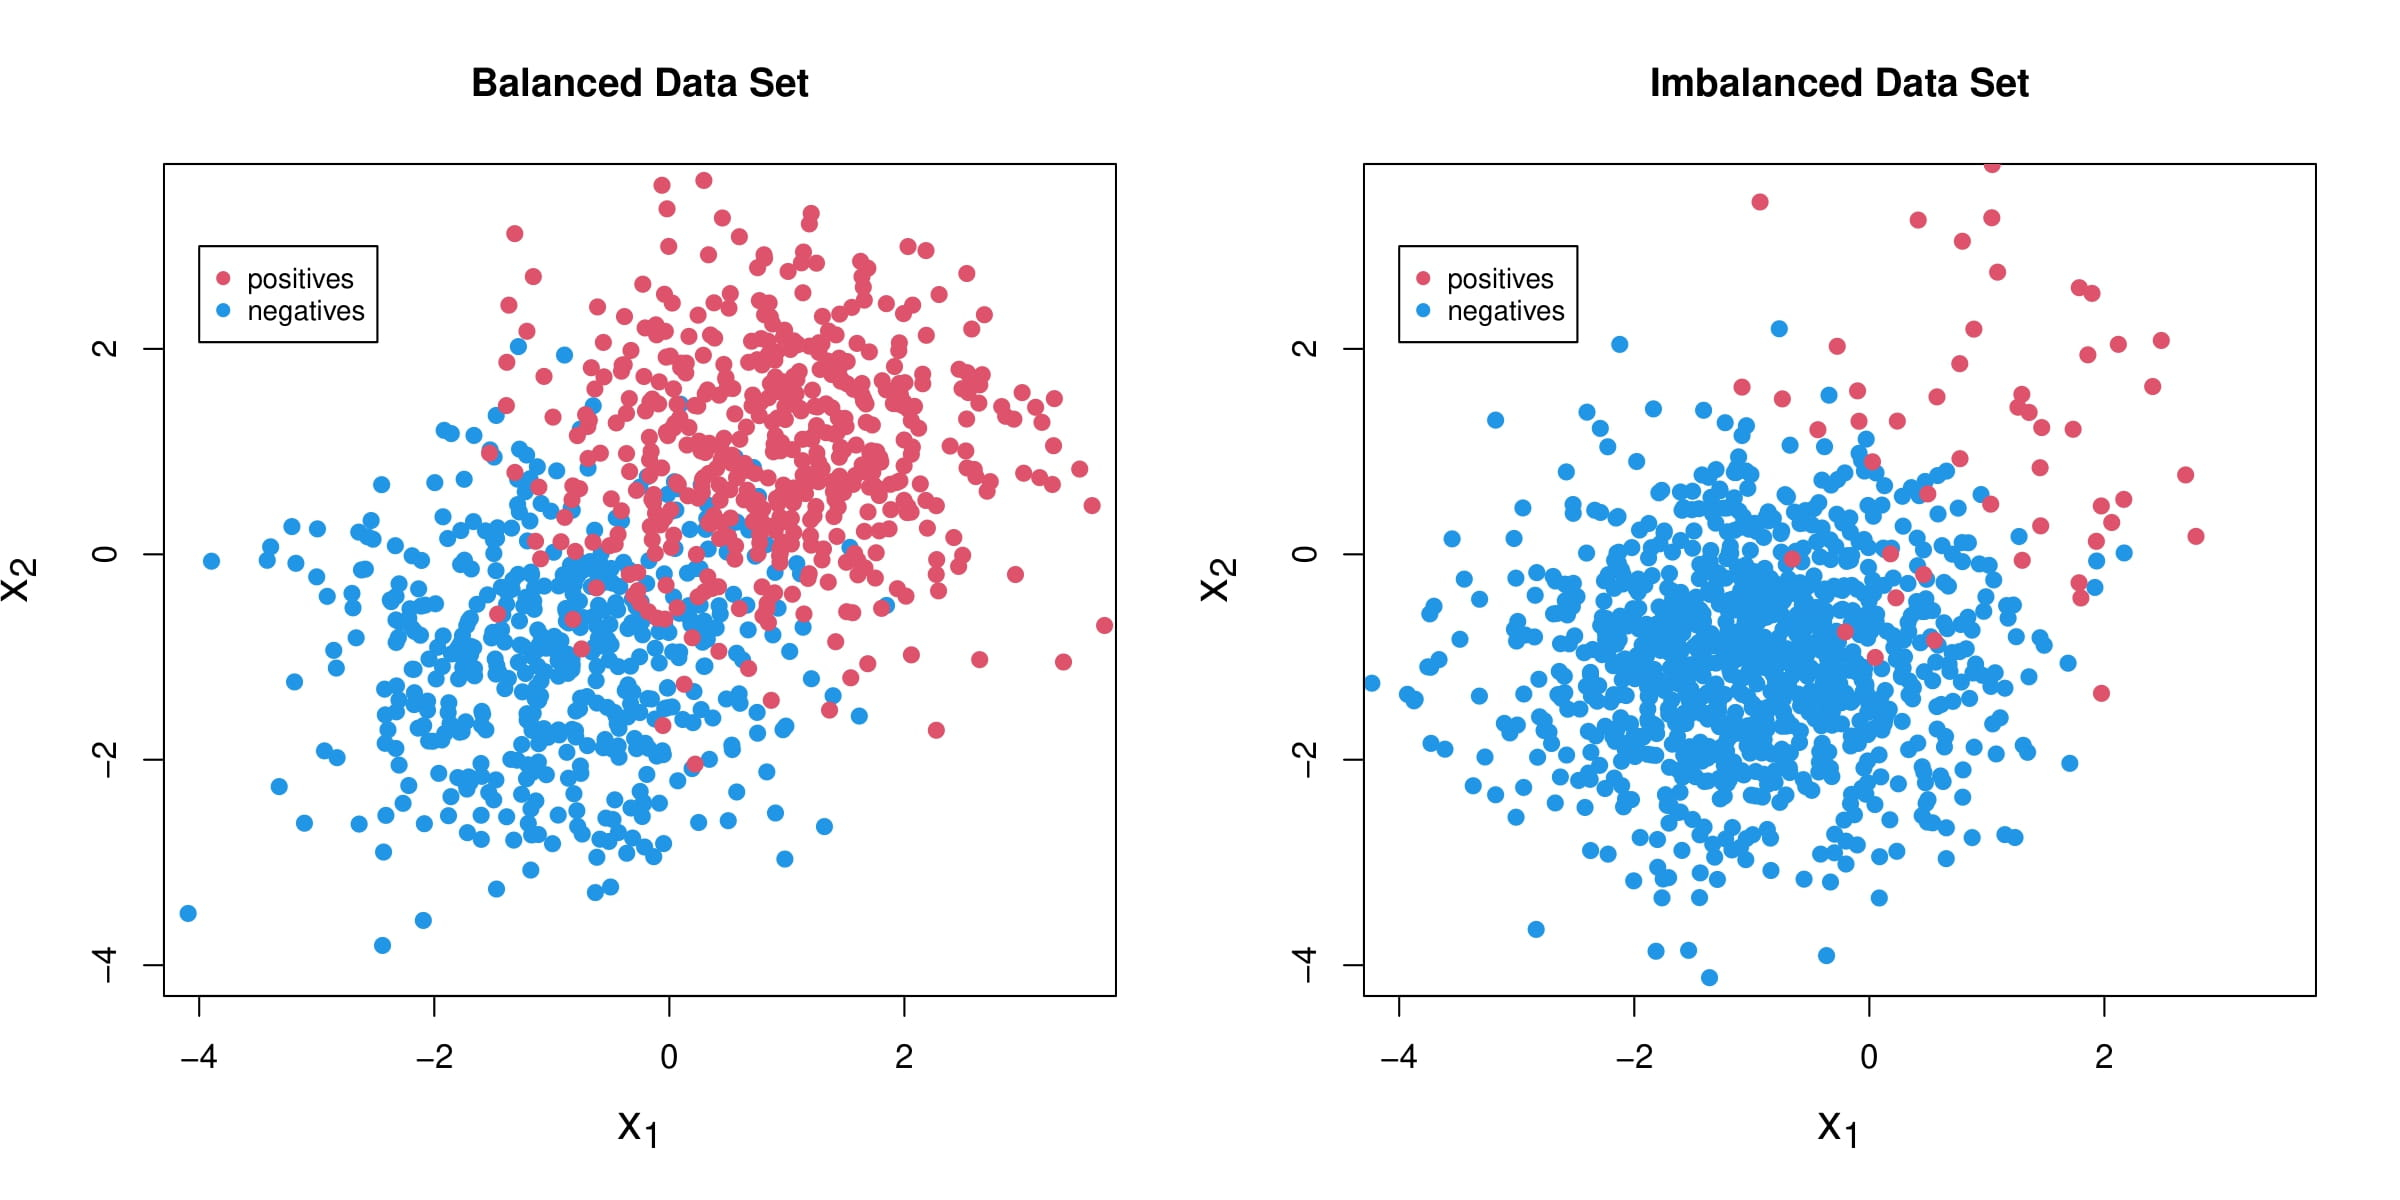
\includegraphics[width=\linewidth]{figure_man/combined_data_plots.jpg}
			\end{figure}
%
\end{frame}

\begin{frame}{Imbalanced Data Sets: Examples}
    \small
    \begin{table}[h]
        \scriptsize
        \centering
        \begin{tabular}{llll}
            \toprule
            \textbf{Domain} & \textbf{Task} & \textbf{Majority Class} & \textbf{Minor Class} \\ [5pt]
            \hline
            Medicine & Predict tumor pathology & Benign &  Malignant \\ [5pt]
            Information retrieval & Find relevant items & Irrelevant items & Relevant items \\ [5pt]
            Tracking criminals & Detect fraud emails & Non-fraud emails & Fraud emails \\ [5pt]
            Weather prediction & Predict extreme weather & Normal weather & Tornado, hurricane \\
            \hline
        \end{tabular}
    \end{table}
    
	\begin{itemize}
        \item Often, the minority class is the more important class.
        \item Imbalanced data can be a source of bias related to concept of fairness. % in ML, e.g.\ more data on white recidivism outcomes than for blacks.
	\end{itemize}

\end{frame}

\frame{
\frametitle{Issues with Evaluating Classifiers}

\begin{itemize}
    \item Ideal case: correctly classify as many instances as possible \\ $\Rightarrow$ High accuracy,	preferably $100\%$.
   % \vspace{10pt}
    
	\item In practice, we often obtain on imbalanced data sets: \textbf{good} performance on the \textbf{majority} class(es), a \textbf{poor} performance on the \textbf{minority} class(es). 	
    %\vspace{10pt}

	\item Reason: the classifier is biased towards the \textbf{majority} class(es), as predicting the majority class pays off in terms of accuracy.
    %\vspace{10pt}

	\item Focusing only on accuracy can lead to bad performance on minority class. 
    %\vspace{10pt}
        \item Example:
		\begin{itemize}
			\small
			\item Assume that only 0.5\% of the patients have a disease,	
			\item Always predicting ``no disease'' leads to accuracy of 99.5\% %\\	$\Rightarrow$ Optimal policy would be no treating anybody		
		\end{itemize}
\end{itemize}
%
}

\begin{frame}{Issues with Evaluating Classifiers}
%
			\begin{figure}
				\centering
				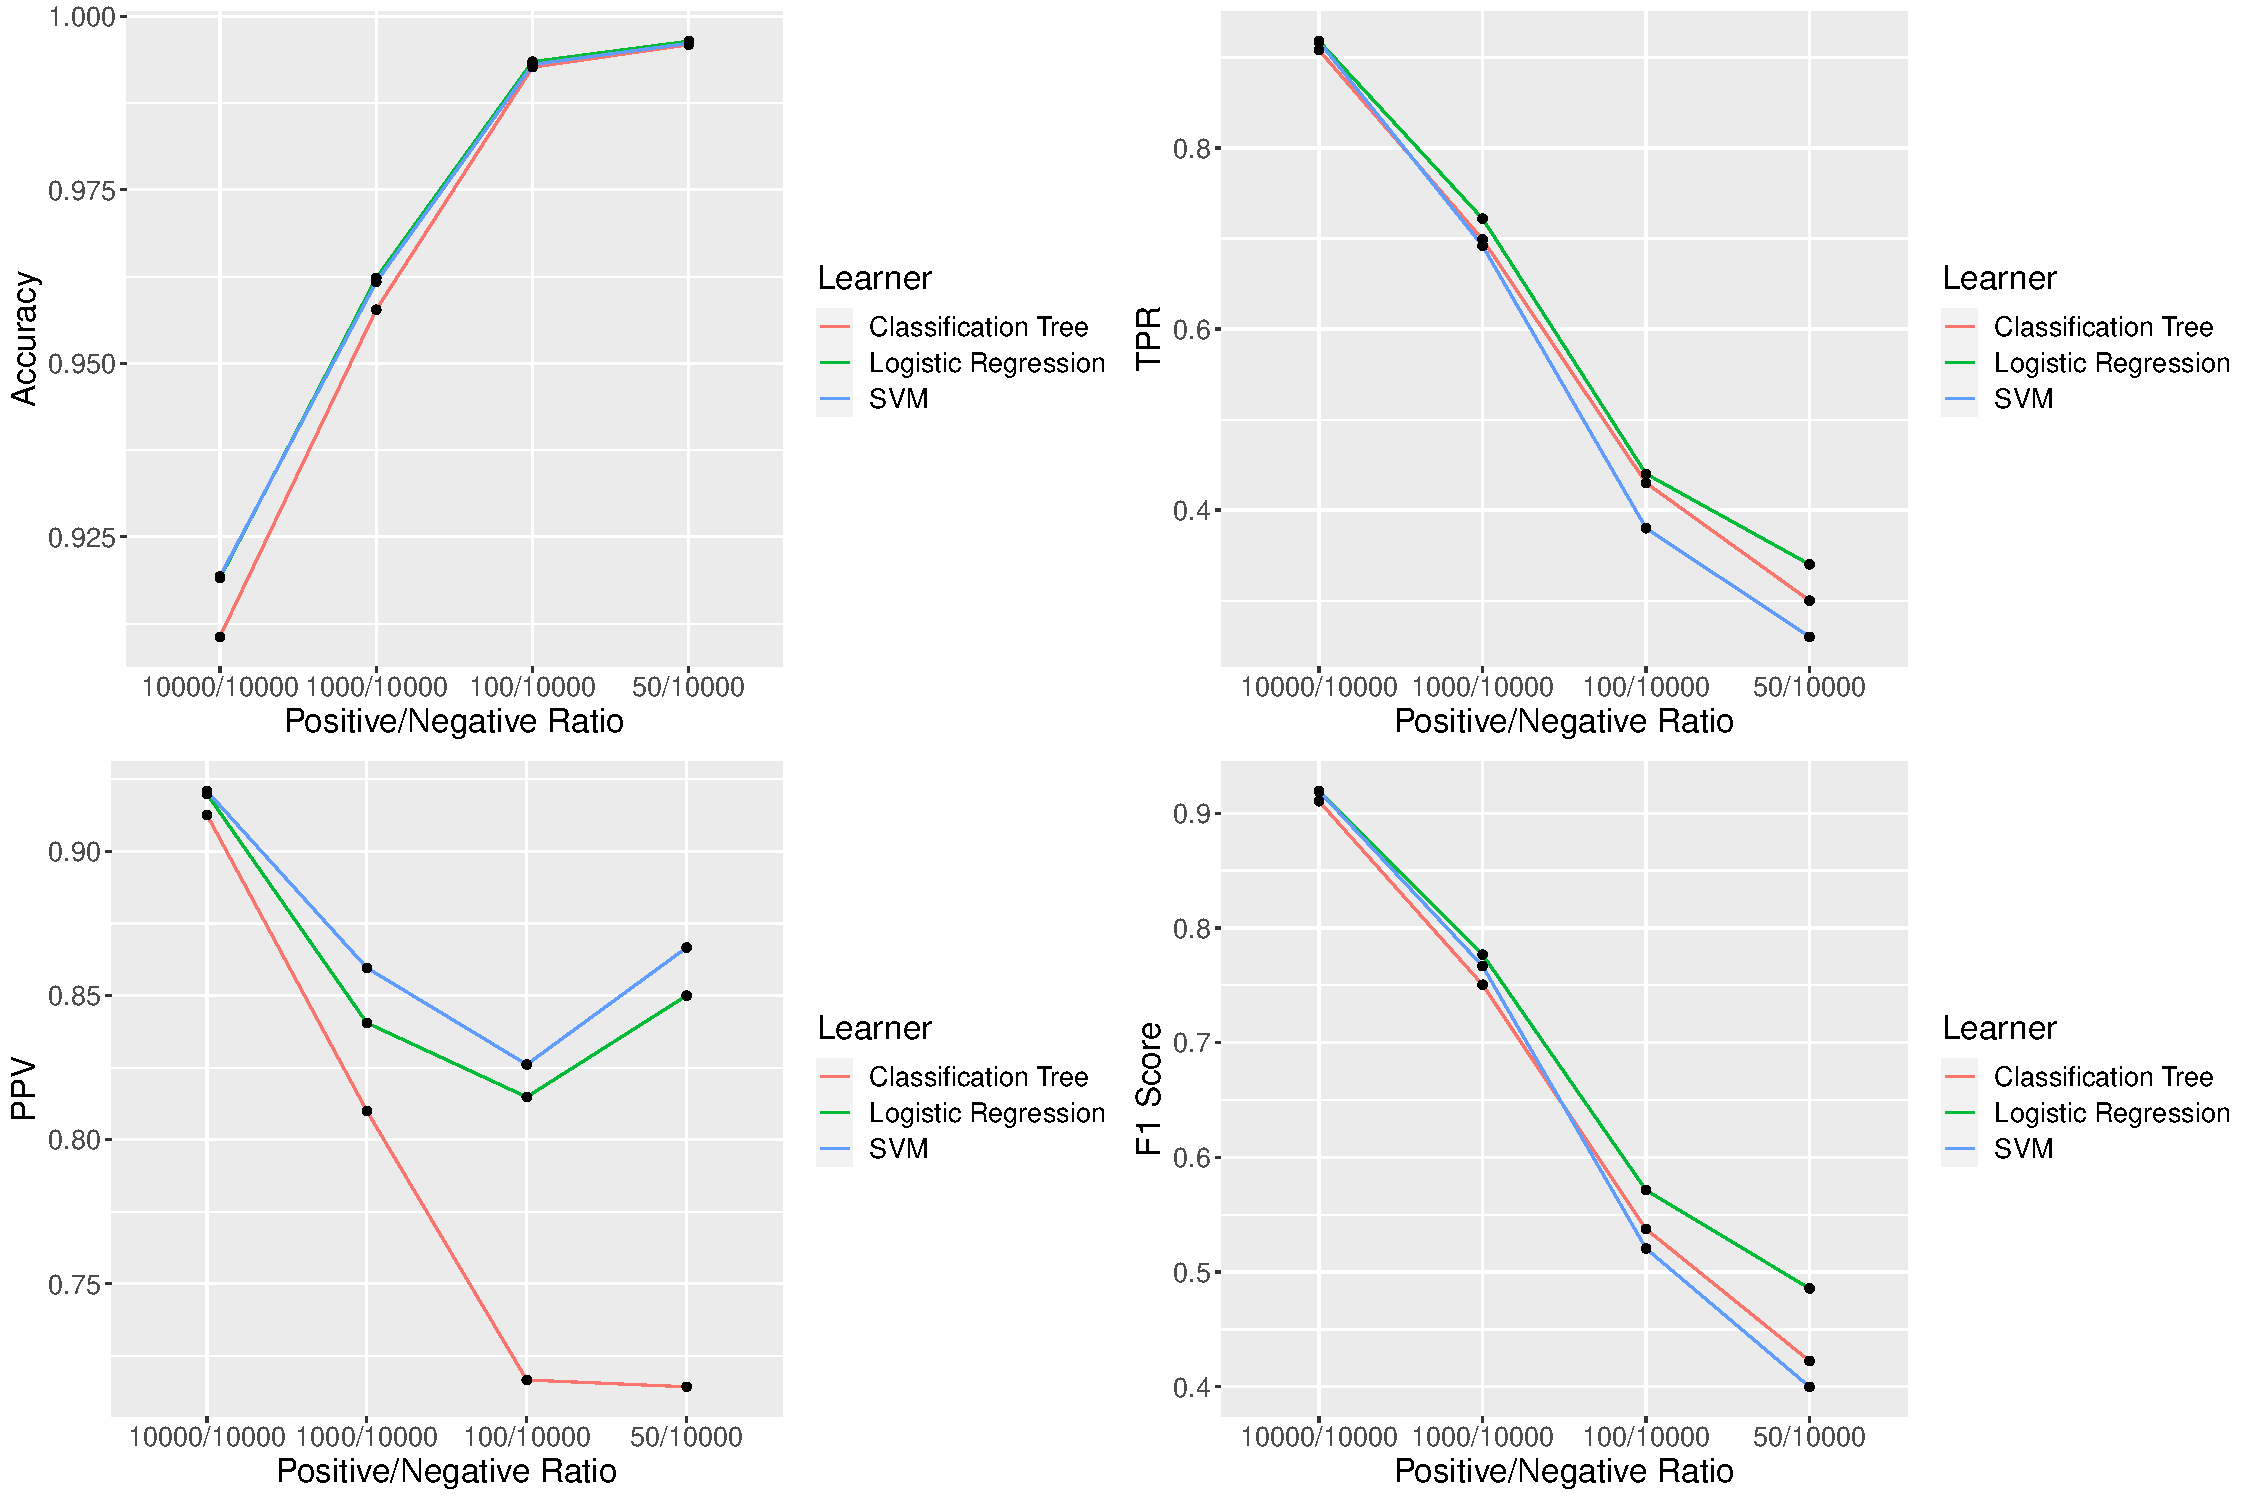
\includegraphics[width=0.8\linewidth]{figure_man/benchmark_plots.pdf}
			\end{figure}
			
			
			\footnotesize
                In each scenario, we have 10.000 obs in the negative class. Number of obs in positive class varies between 10.000, 1.000, 100, and 50. Train classifiers with 10-fold stratified cv. Evaluate via aggregated predictions on test set.
			

%
\end{frame}

\begin{frame}{Possible Solutions}
	%
	\begin{itemize}
        
		\item Ideal performance metric: the learning is \emph{properly} biased towards the minority class(es).	
        %\vspace{20pt}

        \item Imbalance-aware performance metrics:
        \begin{itemize}
            \item G-score
            \item Balanced accuracy
            \item Matthews Correlation Coefficient
            \item Weighted macro $F_1$ score
        \end{itemize}
	\end{itemize}
\end{frame} 


\begin{frame}{Possible Solutions}
%\small
\begin{table}[h]
\footnotesize
    \centering
    \begin{tabular}{p{0.2\textwidth} p{0.4\textwidth} p{0.35\textwidth}}
        \toprule
        \textbf{Approach} & \textbf{Main idea} & \textbf{Remark} \\ [5pt]
        \hline
        Algorithm-level & Bias classifiers towards minority & Special knowledge about classifiers is needed \\ [5pt]
        \hline
        Data-level & Rebalance classes by resampling & No modification of classifiers is needed \\ [5pt]
        \hline
        Cost-sensitive Learning & Introduce different costs for misclassification when learning & Between algorithm- and data-level approaches \\ [15pt]
        \hline
        Ensemble-based & Ensemble learning plus one of three techniques above & - \\ [5pt]
        \bottomrule
    \end{tabular}
\end{table}

\end{frame}


\section{Performance Measures for Imbalanced Data}
% https://github.com/slds-lmu/lecture_advml/blob/main/slides/imbalanced-learning/slides-imbalanced-learning-performance-measures.tex

\begin{frame}{Recap: performance measures for binary classification}
    \footnotesize{
        \begin{itemize}
            \item We encourage readers to first go through \href{https://slds-lmu.github.io/i2ml/chapters/04_evaluation/04-08-measures-classification/}{\beamergotobutton{Chapter 04.08 in I2ML }}.
            \item In binary classification  ($\Yspace = \{-1,+1\}$):

		\end{itemize}
		
		\begin{center}
		\tiny
		\renewcommand{\arraystretch}{1.1}
		\begin{tabular}{cc||cc|c}
			& & \multicolumn{2}{c|}{\bfseries True Class $y$} & \\
			& & $+$ & $-$ & \\ 
			\hline \hline
			\bfseries Classification     & $+$ & TP & FP & $\rho_{PPV} = \frac{\tp}{\tp + \fap}$\\
			$\yh$ & $-$ & FN & TN & $\rho_{NPV} = \frac{\tn}{\fan + \tn}$\\
			\hline
			& & $\rho_{TPR} = \frac{\tp}{\tp + \fan}$ & $\rho_{TNR} = \frac{\tn}{\fap + \tn}$ & $\rho_{ACC} = \frac{\tp+ \tn}{\text{TOTAL}}$
		\end{tabular}
		\renewcommand{\arraystretch}{1}
        \end{center}

        \begin{itemize}
            \item $F_1$ score balances Recall ($\rho_{TPR}$) and Precision ($\rho_{PPV}$):
            $$\rho_{F_1} = 2 \cdot \cfrac{\rho_{PPV} \cdot \rho_{TPR}}{\rho_{PPV} + \rho_{TPR}}$$
            
            \item Note that $\rho_{F_1}$ does not account for TN.
            
            \item Does $\rho_{F_1}$ suffer from data imbalance like accuracy does?
            % See section 4.2 from "An introduction to ROC analysis" by Fawcett (2006) for an explanation: "If the proportion of positive to negative instances changes ina test set, the ROC curves will not change. To see why this is so, consider the confusion matrix in Figure 1. Note that the class distribution - the proportion of positive to negativ einstances -is the relationship of the left (+) column tot he right (-) column. Any performance metric that uses values from both columns will be inherently sensitive to class skews. Metrics such as accuracy , precision, lift and Fscores use values from both columns of the confusion matrix.
        \end{itemize}
            
    }
    
\end{frame}


\begin{frame}{$F_1$ Score in Binary classification}
	\footnotesize{
	
    	\begin{minipage}[c]{0.5\textwidth}
    		$F_1$ is the \textbf{harmonic mean} of $\rho_{PPV}$ \& $\rho_{TPR}$. \\
    		$\rightarrow$ Property of harmonic mean: tends more towards the \textbf{lower} of two combined values.
    	\end{minipage}%
    	\begin{minipage}[c]{0.5\textwidth}
    		\centering
    		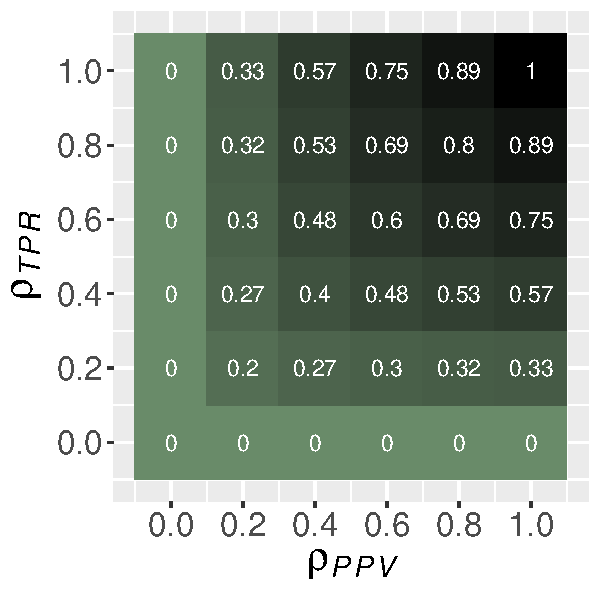
\includegraphics[width=0.8\textwidth]{figure/f1_score_plot.pdf}
    	\end{minipage}
	
    	\begin{itemize}
    		\item A model with $\rho_{TPR} = 0$ %(no pos. instance predicted as pos.) 
      or 
    		$\rho_{PPV} = 0$ %(no TP among the predicted) 
      has $\rho_{F_1} = 0$.
      
    		\item Always predicting \enquote{negative}: $\rho_{TPR} = \rho_{F_1} = 0$
      
    		\item Always predicting \enquote{positive}: $\rho_{TPR} = 1 \Rightarrow \rho_{F_1} = 2 \cdot \rho_{PPV} / 
    		(\rho_{PPV} + 1) = 2 \cdot \np / (\np + n)$,\\ 
    		$\leadsto$ small when $\np (= TP + FN = TP)$  is small.
    
            \item Hence, $F_1$ score is more robust to data imbalance than accuracy.
      
    	\end{itemize}
	}
\end{frame}

\begin{frame}{$F_\beta$ in Binary classification}
    \footnotesize{
	
    	\begin{minipage}[c]{0.49\textwidth}
            \begin{itemize}
                \item $F_1$ puts equal weights to $\frac{1}{\rho_{PPV}}$ \& $\frac{1}{\rho_{TPR}}$ because $F_1 = \frac{2}{\frac{1}{\rho_{PPV}} + \frac{1}{\rho_{TPR}}}$.
                
                \item $F_\beta$ puts $\beta^2$ times of weight to $\frac{1}{\rho_{TPR}}$:
                    \begin{equation*}
                        \begin{aligned}
                            F_\beta &= \frac{1}{\frac{\beta^2}{1 + \beta^2} \cdot \frac{1}{\rho_{TPR}} + \frac{1}{1 + \beta^2} \cdot \frac{1}{\rho_{PPV}}} \\
                            &= (1 + \beta^2) \cdot \frac{\rho_{PPV} \cdot \rho_{TPR}}{\beta^2 \rho_{PPV} + \rho_{TPR}}
                        \end{aligned}
                    \end{equation*}
            \end{itemize}
    	\end{minipage}
    	\begin{minipage}[c]{0.49\textwidth}
    		\centering
    		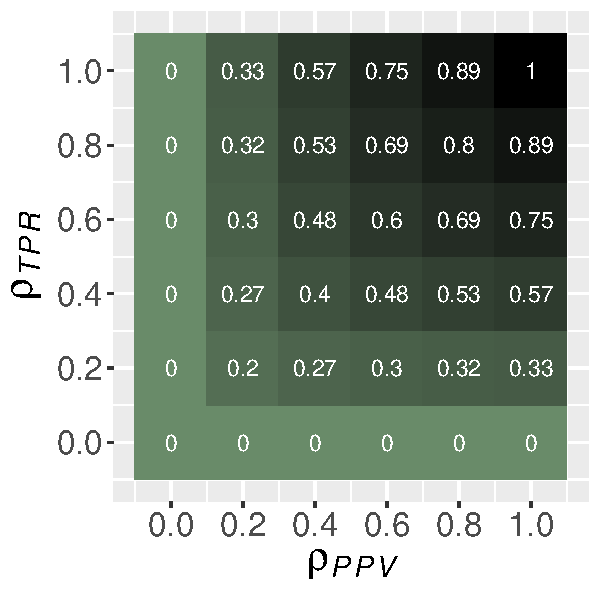
\includegraphics[width=0.8\textwidth]{figure/f1_score_plot.pdf}
    	\end{minipage}
    	
    	\begin{itemize}
    		\item $\beta \gg 1 \ \leadsto \ F_\beta \approx \rho_{TPR}$;
            \item $\beta \ll 1 \ \leadsto \ F_\beta \approx \rho_{PPV}$.
      
    	\end{itemize}

    }
    
\end{frame}


\begin{frame}{G Score and G Mean}
	\footnotesize{
    	\begin{minipage}[c]{0.49\textwidth}
        	\begin{itemize}
        		\item G score uses geometric mean: 
        		$$\rho_{G} = \sqrt{\rho_{PPV} \cdot \rho_{TPR}}$$

        		\item Geometric mean tends more towards the \textbf{lower} of the two combined values.
                \item Geometric mean is \textbf{larger} than harmonic mean.
        	\end{itemize}
        \end{minipage}
        \begin{minipage}[c]{0.49\textwidth}
        	\centering
        	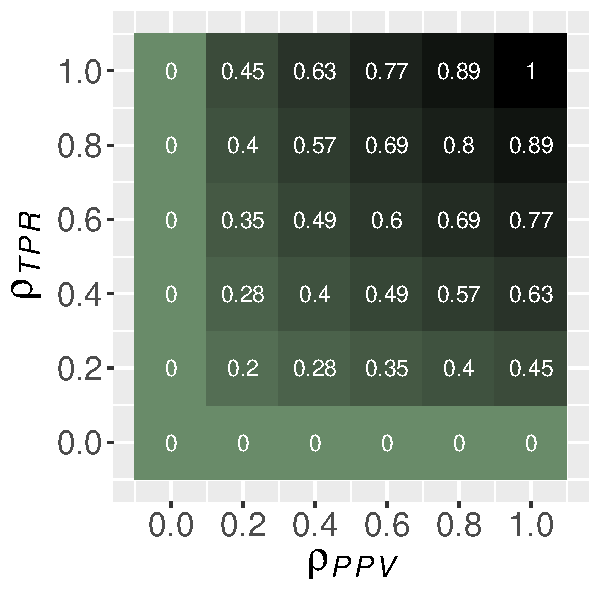
\includegraphics[width=0.8\textwidth]{figure/g_score_plot.pdf}
        \end{minipage}

        \begin{itemize}
        	\item Closely related is the G mean:
        	$$\rho_{Gm} = \sqrt{\rho_{TNR} \cdot \rho_{TPR}}.$$
        	It also considers \textbf{TN}.
    
        	\item Always predicting \enquote{negative}: $\rho_{G} = \rho_{Gm}  = 0 \leadsto$ Robust to data imbalance!
        \end{itemize}
}
\end{frame}



\begin{frame}{Balanced Accuracy}
	\footnotesize{
	
    	\begin{minipage}[c]{0.49\textwidth}
    		\begin{itemize}
    			\item Balanced accuracy (BAC) balances $\rho_{TNR}$ and $\rho_{TPR}$: 
    			$$\rho_{BAC} = \frac{\rho_{TNR} + \rho_{TPR}}{2}$$

    			%\item  It tends more towards the \textbf{higher} of two combined values.
    		\end{itemize}
    	\end{minipage}
    	\begin{minipage}[c]{0.49\textwidth}
    		\centering
    		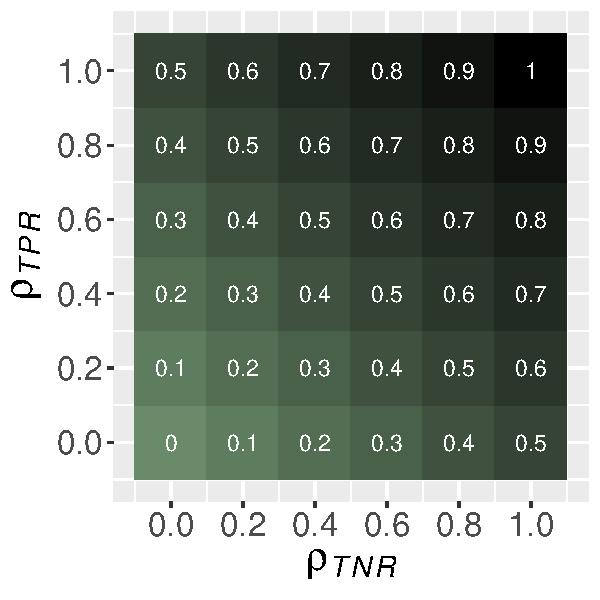
\includegraphics[width=0.8\textwidth]{figure/bac_plot.pdf}
    	\end{minipage}

    	\begin{itemize}
    		\item If a classifier attains high accuracy on both classes or the data set is almost balanced, then $\rho_{BAC} \approx \rho_{ACC}$.
            \vspace{20pt}
            
    		\item However, if a classifier always predicts ``negative'' for an imbalanced data set, i.e. $n_+  \ll n_-,$ then $\rho_{BAC} \ll \rho_{ACC}$. It also considers TN.
    
    	\end{itemize}
    }
\end{frame}

\begin{frame}{Matthews Correlation Coefficient}

	\small{
    	\begin{itemize}
    
            \item Recall: Pearson correlation coefficient (PCC): 
                $$\corr(X, Y) = \frac{\cov(X, Y)}{\sigma_{X} \sigma_{Y}}$$
    		\item View ``predicted'' and ``true'' classes as two binary random variables.
      
            \item Using entries in confusion matrix to estimate the PCC, we obtain MCC:
    	
    		$$   \rho_{MCC} = \frac{TP\cdot TN - FP \cdot FN}{\sqrt{(TP+FN)(TP+FP)(TN+FN)(TN+FP)}}$$
    
            \item In contrast to other metrics: 
            \begin{itemize}
                \footnotesize
                \item MCC uses all entries of the confusion matrix;
                \item MCC has value in $[-1,1]$.
            \end{itemize}
    		
        \end{itemize}
    	
	}
\end{frame}

\begin{frame}{Matthews Correlation Coefficient}
    \small{
        $$   \rho_{MCC} = \frac{TP\cdot TN - FP \cdot FN}{\sqrt{(TP+FN)(TP+FP)(TN+FN)(TN+FP)}}$$

        \begin{itemize}
            \item $\rho_{MCC} \approx 1$ $\leadsto$ nearly zero error $\leadsto$ good classification, i.e., strong correlation between predicted and true classes.
            \vspace{10pt}
    	
            \item $\rho_{MCC} \approx 0$ $\leadsto$ no correlation, i.e., not better than random guessing.
            \vspace{10pt}
    	
            \item $\rho_{MCC} \approx -1$ $\leadsto$ reversed classification, i.e., switch labels.
            \vspace{10pt}
    
            \item Previous measures requires defining positive class. But MCC does not depend on which class is the positive one.
            
        \end{itemize}
         
    }
    
\end{frame}


\begin{frame}{Multiclass Classification}
	\small{
		\begin{center}
			\tiny
			\begin{tabular}{cc|>{\centering\arraybackslash}p{8em}>{\centering\arraybackslash}p{8em}>{\centering\arraybackslash}p{5em}>{\centering\arraybackslash}p{8em}}
				& & \multicolumn{4}{c}{\bfseries True Class $y$} \\
				& & $1$ & $2$ & $\ldots$ & $g$  \\
				\hline
				\bfseries Classification     & $1$ & $n_{11}$  &  $n_{12}$  & $\ldots$ &  $n_{1g}$ \\
				& & (True 1's) & (False 1's for 2's) & $\ldots$ &  (False 1's for $g$'s)  \\
				& $2$ &  $n_{21}$  &  $n_{22}$  & $\ldots$ & $n_{2g}$  \\
				$\yh$ & & (False 2's for 1's) & (True 2's) & $\ldots$ &  (False 2's for $g$'s)  \\
				& $\vdots$ & $\vdots$ & $\vdots$ & $\ldots$ & $\vdots$ \\
				& $g$ & $n_{g1}$ & $n_{g2}$  & $\ldots$ &  $n_{gg}$\\
				& & (False $g$'s for 1's) & (False $g$'s for 2's) & $\ldots$ &  (True $g$'s)  \\
			\end{tabular}
		\end{center}
		
		\begin{itemize}
			\item $n_{ji}$: the number of $i$ instances classified as $j$.

            \item $n_i = \sum_{j=1}^g n_{ji}$ the total number of $i$ instances.

            \item \textbf{Class-specific} metrics:
                \begin{itemize}
                    \small
                    
                    \item True positive rate (\textbf{Recall}): $\rho_{TPR_i} = \frac{n_{ii}}{n_i}$
    
                    \item True negative rate $\rho_{TNR_i} = \frac{\sum_{j\neq i}n_{jj}}{n-n_i}$ 
    
                    \item Positive predictive value (\textbf{Precision}) $\rho_{PPR_j} = \frac{n_{jj}}{\sum_{i=1}^g n_{ji}}$.
                    
                \end{itemize}

		\end{itemize}
	}
\end{frame}


\begin{frame}{Macro $F_1$ Score}
	
	\small{

    	\begin{itemize}
    
    		\item Average over classes to obtain a single value:
            $$\rho_{mMETRIC} = \frac{1}{g}\sum_{i=1}^g \rho_{METRIC_i},$$
            where $METRIC_i$ is a class-specific metric such as $PPV_i$, $TPR_i$ of class $i$.
    		
    	
    		\item With this, one can simply define a \textbf{macro} $F_1$ score:
    	
    		$$\rho_{mF_1} = 2 \cdot \cfrac{\rho_{mPPV} \cdot \rho_{mTPR}}{\rho_{mPPV} + 
    			\rho_{mTPR}}$$
    
    		\item Problem: each class equally weighted $\leadsto$ class sizes are not considered.
    
            \item How about applying different weights to the class-specific metrics?

    	\end{itemize}
	}
\end{frame}

\begin{frame}{Weighted Macro $F_1$ Score}

	\small{

    	\begin{itemize}
    
    		\item For imbalanced data sets, give \textbf{more weights} to \textbf{minority} classes.
      
            \item $w_1,\ldots,w_g \in[0,1]$  such that $w_i > w_j$ iff $n_i < n_j$ and $\sum_{i=1}^g w_i = 1.$
    
            $$\rho_{wmMETRIC} = \frac{1}{g}\sum_{i=1}^g \rho_{METRIC_i} w_i,$$
            where $METRIC_i$ is a class-specific metric such as $PPV_i$, $TPR_i$ of class $i$.
    	 
    		\item Example: $w_i = \frac{n - n_i}{(g-1)n}$ are suitable weights.
    
    		\item Weighted macro $F_1$ score:	
    		$$\rho_{wmF_1} = 2 \cdot \frac{\rho_{wmPPV} \cdot \rho_{wmTPR}}{\rho_{wmPPV} + \rho_{wmTPR}}$$
      
    		\item This idea gives rise to a weighted macro G score or weighted BAC.
    	
    		\item \textbf{Usually}, weighted $F_1$ score uses $w_i = n_i/n$. However, for imbalanced data sets this would \textbf{overweight} majority classes.
    
    	\end{itemize}
	}
\end{frame}


\begin{frame}{Other Performance Measures}

	\small{

		\begin{itemize}
		
			\item ``Micro'' versions, e.g., the micro $TPR$ is $\frac{\sum_{i=1}^g TP_i}{\sum_{i=1}^g TP_i + FN_i}$ 
            \vspace{10pt}
		
			\item MCC can be extended to:
			
			$$   \rho_{MCC} = \frac{ n  \sum_{i=1}^g n_{ii} -  \sum_{i=1}^g \hat n_i n_i}{\sqrt{ (n^2 - \sum_{i=1}^g \hat n_i^2)(n^2 - \sum_{i=1}^g n_i^2)  }},$$

			where $\hat n_i = \sum_{j=1}^g n_{ij}$ is the total number of instances classified as $i.$
            \vspace{10pt}
        
		
			\item Cohen's Kappa or Cross Entropy (see Grandini et al.\ (2021)) treat "predicted" and "true" classes as two discrete random variables.
		
		\end{itemize}
	}
\end{frame}


\begin{frame}{Which Performance Measure to use?}

	\small{

		\begin{itemize}

            \item Since different measures focus on other characteristics $\leadsto$ No golden answer to this question.
	
			\item Depends on application and importance of characteristics.

			\item However, it is clear that accuracy usage is inappropriate if the data set is imbalanced. $\leadsto$ Use alternative metrics.

			\item Be careful with comparing the absolute values of the different measures, as these can be on different ``scales'', e.g.,\ MCC and BAC. 

                \item Area under the ROC curve is also immune against class imbalance.
	
		\end{itemize}
	}
\end{frame}


% https://github.com/slds-lmu/lecture_advml/blob/main/slides/imbalanced-learning/slides-imbalanced-learning-cost-sensitive-learning-1.tex
% https://github.com/slds-lmu/lecture_advml/blob/main/slides/imbalanced-learning/slides-imbalanced-learning-cost-sensitive-learning-2.tex
% https://github.com/slds-lmu/lecture_advml/blob/main/slides/imbalanced-learning/slides-imbalanced-learning-cost-sensitive-learning-3.tex

\section{Cost-Sensitive Learning}

\begin{frame}{Cost-Sensitive learning: In a Nutshell}
	%	
	\scriptsize{

		\begin{itemize}
		
    		\item Cost-sensitive learning: 
                \begin{itemize}
                    \scriptsize
                    \item Classical learning: data sets are balanced, and all errors have equal costs
                    \item We now assume given, unequal cost
                    \item And try to minimize them in expectation

                \end{itemize}
    		
    		\item Applications:
      
    		\begin{itemize}
    			\scriptsize	
    			\item Medicine --- Misdiagnosing as healthy vs. having a disease
    			\item (Extreme) Weather prediction ---  Incorrectly predicting that no hurricane occurs 
    			\item Credit granting --- Lending to a risky client vs. not lending to a trustworthy client.
    		\end{itemize}
         
		
		\end{itemize}
        \vspace{15pt}

        \begin{minipage}{0.49\textwidth}
            \begin{table}[]
                \centering
                \begin{tabular}{p{1cm}c|cc}
                    & &\multicolumn{2}{c}{Truth} \\
                    & & Default & Pays Back  \\
                    \hline
                    \multirow{2}{*}{\parbox{1cm}{Pred.}} & Default & 0 & $ 10 $\\
                    & Pays Back & $1000$ & $0$   \\
                \end{tabular}
            \end{table}
        \end{minipage}
        \hfill
        \begin{minipage}{0.49\textwidth}
            \begin{itemize}
                \scriptsize
                \item In these examples, \textbf{the costs of a false negative is much higher than the costs of a false positive}.
                \vspace{15pt}
                
                \item In some applications, the costs are \textbf{unknown} $\leadsto$ need to be specified by experts, or be learnt.
            \end{itemize}   
        \end{minipage}
		
	}
\end{frame}

\begin{frame}{Cost matrix}
%	
%	
	\begin{itemize}
%		
		\item Input: cost matrix $\mathbf{C}$ 
	\end{itemize}
	%	
	\begin{center}
		\tiny
		\begin{tabular}{cc|>{\centering\arraybackslash}p{8em}>{\centering\arraybackslash}p{8em}>{\centering\arraybackslash}p{5em}>{\centering\arraybackslash}p{8em}}
			& & \multicolumn{4}{c}{\bfseries True Class $y$} \\
			&  & $1$ & $2$ & $\ldots$ & $g$  \\
			\hline
			\bfseries Classification     & $1$ & $C(1,1)$  &  $C(1,2)$  & $\ldots$ &  $C(1,g)$ \\
			& $2$ &  $C(2,1)$  &  $C(2,2)$  & $\ldots$ & $C(2,g)$  \\
            $\yh$ & & & & & \\
			& $\vdots$ & $\vdots$ & $\vdots$ & $\ldots$ & $\vdots$ \\
			& $g$ & $C(g,1)$ & $C(g,2)$  & $\ldots$ &  $C(g,g)$\\
		\end{tabular}
	\end{center}
	%	
	\begin{itemize}
		%		
		\item $C(j,k)$ is the cost of classifying class $k$ as $j,$ 
  \item 0-1-loss would simply be: $C(j,k) = \mathds{1}_{[ j \neq k ]}$
		
		\item $\mathbf{C}$ designed by experts with domain knowledge
		\begin{enumerate}
            \item Too low costs: not enough change in model, still costly errors
            \item Too high costs: might never predict costly classes
		\end{enumerate}
		
	\end{itemize}


\end{frame}


\begin{frame}{Cost matrix for Imbalanced Learning}
		\begin{itemize}			
	 
			\item Common heuristic for imbalanced data sets: 
	
			\begin{itemize}
                \item $C(j,k) = \frac{n_j}{n_k}$ with $n_k  \ll n_j$,\\
                misclassifying a minority class $k$ as a majority class $j$
		
				\item $C(j,k) = 1$ with $n_j \ll n_k$,\\
    misclassifying a majority class $k$ as a minority class $j$
			
				\item 0 for a correct classification 
			
			\end{itemize}
\vspace{1cm}
    		\item Imbalanced binary classification: \\
            \begin{table}[]
                \centering
                \begin{tabular}{cc|cc}
                    & &\multicolumn{2}{c}{True class} \\
                    & & $y=1$ & $y=-1$  \\
                    \hline
                    \multirow{2}{*}{\parbox{0.5cm}{Pred. class}}& $\hat y$ = 1     & $0$                & $ 1 $\\
                    & $\hat y$ = -1 & $ \frac{n_-}{n_+} $              &  $0$   \\
                \end{tabular}
            \end{table}
    		

            \item So: much higher costs for FNs
        \end{itemize}
		
\end{frame}

\begin{frame}{Minimum expected Cost Principle}


		\begin{itemize}
		
			\item Suppose we have:
            \begin{itemize}
                \item a cost matrix $\mathbf{C}$
                
                \item knowledge of the true posterior $p(\cdot ~|~ \xv)$
            \end{itemize}

            % \item How to classify given $\xv$: 
            % \begin{itemize}
            %     \footnotesize
            %     \item Compute cost for classifying $\xv$ as $i$. (infeasible to directly compute.)
            %     \vspace{10pt}
                
            %     \item $\leadsto$ Marginalize over ``true'' class $j$.
            %     \vspace{10pt}
            % \end{itemize}

			\item Predict class j with smallest expected costs when marginalizing over true classes:
   %, where the expected costs of a class $i\in\{1,\ldots,g\}$ is
	
			$$ 	\E_{K \sim p(\cdot ~|~ \xv)}( C(j,K) ) = \sumkg p(k ~|~ \xv) C(j,k)	$$
	
		\end{itemize}

    \begin{itemize}
        \item If we trust a probabilistic classifier, we can convert its scores to labels:
        % $f$ which uses a probabilistic score function $\pi:\Xspace \to [0,1]^g$ with $\pi(\xv) = (\pi(\xv)_1,\ldots,\pi(\xv)_g)^\top$ and $\sum_{j=1}^g \pi(\xv)_j = 1$ for the classification, then one can easily modify $h$ to take the expected costs into account:
		$$  \hx := \argminlim_{j=1,\ldots,g} \sumkg 	\pikx C(j,k). $$
 
%        \item For $\xv$, making prediction $i$ means \textbf{acting as if $i$ is the true class of $\xv$.}
        
        \item Can be better to take a less probable class (\href{https://dl.acm.org/doi/10.5555/1642194.1642224}{\beamergotobutton{Elkan et. al. 2001}})

        % \item Now consider: 
        % \begin{itemize}
        %     \footnotesize
        %     \item If we learnt a binary classifier: $p(1 ~|~ \xv) = \pi(\xv)_1$ and $p(-1 ~|~ \xv) = \pi(\xv)_2$,
        %     \item Under what condition should we predict $\xv$ as class $1$?
        % \end{itemize}
    \end{itemize}
\end{frame}


\begin{frame}{Optimal Threshold for Binary Case 1/2}
    \begin{itemize}
            \item Optimal decisions do not change if 
            \begin{itemize}
                \item $\mathbf{C}$ is multiplied by positive constant
                \item $\mathbf{C}$ is added with constant shift
            \end{itemize}

            \item Scale and shift $\mathbf{C}$ to get simpler $\mathbf{C}^\prime$: 
            \begin{table}[]
                \centering
                    \begin{tabular}{cc|cc}
        			& &\multicolumn{2}{c}{True class} \\
        			& & $y=1$ & $y=-1$  \\
        			\hline
        			\multirow{2}{*}{\parbox{0.5cm}{Pred.  class}} & $\hat y$ = 1 & $C^\prime(1,1)$ & $1$ \\
        			& $\hat y$ = -1 & $C^\prime(-1, 1)$ & 0\\
                \end{tabular}
            \end{table}
            where 
            \begin{itemize}
                \item $C^\prime (-1, 1) = \frac{C(-1, 1) - C(-1, -1)}{C(1, -1) - C(-1, -1)}$
                \item $C^\prime (1, 1) = \frac{C(1, 1) - C(-1, -1)}{C(1, -1) - C(-1,-1)}$
            \end{itemize}
    \end{itemize}
\end{frame}
\begin{frame}{Optimal Threshold for Binary Case 2/2}
            \begin{itemize}
            \item We predict $\xv$ as class $1$ if 
            \begin{align*}
                \E_{K \sim p(\cdot ~|~ \xv)}( C^\prime(1,K) )  \leq \E_{K \sim p(\cdot ~|~ \xv)}( C^\prime(-1,K) ) \\
            \end{align*}

			\item Let's unroll the expected value and use $\mathbf{C}^\prime$:
            % need this footnotsize operation, otherwise the first line will be very long.
            \footnotesize{
    			\begin{align*}	
                    & p(-1 ~|~ \xv ) C^\prime(1,-1)  + 	p(1 ~|~ \xv ) C^\prime(1,1) \leq  p(-1 ~|~ \xv ) C^\prime(-1,-1)  + 	p(1 ~|~ \xv ) C^\prime(-1,1)  \\ 
                    &\Rightarrow [1 - p(1 ~|~ \xv)] \cdot 1 + p(1 ~|~ \xv) C^\prime(1, 1) \leq p(1 ~|~ \xv) C^\prime(-1, 1) \\
                    &\Rightarrow p(1 ~|~ \xv) \geq \frac{1}{C^\prime(-1, 1) - C^\prime(1, 1) + 1} \\
                    &\Rightarrow p(1 ~|~ \xv) \geq \frac{C(1, -1) - C(-1, -1)}{C(-1, 1) - C(1, 1) + C(1, -1) - C(-1, -1)} = c^*
    			\end{align*}
            }
		
            \item If even $C(1, 1) = C(-1, -1) = 0 $, we get:
            \begin{align*}
                p(1 ~|~ \xv) \geq \frac{C(1, -1)}{C(-1, 1) + C(1, -1)} = c^{*}
            \end{align*}	
            
            \item Optimal threshold $c^*$ for probabilistic classifier 
            
            $$   \hx := 2 \cdot \mathds{1}_{[ \pi(\xv) \geq c^*]} -1 $$
							
		\end{itemize}
\end{frame}



%\begin{frame}{MetaCost: Example}
%	%	
%	\small{
%		\begin{itemize}
%			%		
%			\item We compare C4.5 (decision tree) with MetaCost using C4.5 for the \href{http://staffwww.itn.liu.se/~aidvi/courses/06/dm/
%				labs/heart-c.arff}{heart data set}  in \href{ http://www.cs.waikato.ac.nz/ml/weka/}{Weka}. 
%			%		
%			\item The cost matrix $\mathbf{C}$ is 
%			
%			\begin{center}
%				\begin{tabular}{cc|cc}
%					& &\multicolumn{2}{c}{True class} \\
%					& & $y=1$ & $y=-1$  \\
%					\hline
%					\multirow{2}{*}{\parbox{0.3cm}{Pred.  class}}& $\hat y$ = 1     & $0$                & $ 1 $\\
%					& $\hat y$ = -1 & $ 4 $              &  $0$   \\
%				\end{tabular}
%			\end{center}
%		
%			\item The resulting confusion matrices are 
%			
%						
%			\begin{center}
%				\begin{tabular}{cc|cc}
%					& &\multicolumn{2}{c}{True class} \\
%					& MetaCost & $y=1$ & $y=-1$  \\
%					\hline
%					\multirow{2}{*}{\parbox{0.3cm}{Pred.  class}}& $\hat y$ = 1     & $104$                & $ 21 $\\
%					& $\hat y$ = -1 & $ 61 $              &  $117$   \\
%				\end{tabular}
%							\begin{tabular}{cc|cc}
%				& &\multicolumn{2}{c}{True class} \\
%				& C4.5 & $y=1$ & $y=-1$  \\
%				\hline
%				\multirow{2}{*}{\parbox{0.3cm}{Pred.  class}}& $\hat y$ = 1     & $138$                & $ 40 $\\
%				& $\hat y$ = -1 & $ 27$              &  $98$   \\
%			\end{tabular}
%			\end{center}
%		
%		
%			%		
%			\item The total cost of MetaCost is 145, while C4.5 has total costs of 187. However, MetaCost has $0.729$ correct classifications and C4.5 has $0.779.$ 
%			
%			%		
%		\end{itemize}
%		%
%	}
%	%	
%\end{frame}



%\begin{frame}{Cost-Sensitive Decision Trees}
%	%	
%	\small{
%		\begin{itemize}
%			%		
%			\item 
%			%		
%		\end{itemize}
%		%
%	}
%	%	
%\end{frame}

\begin{frame}{Empirical Thresholding: binary case}
    \begin{itemize}
        \item Theoretical threshold from MECP not always best, due to e.g. wrong model class, finite data, etc.
        \item Simply measure costs on data with different thresholds
        \item Then pick best threshold (Fig.1 in \href{https://www.aaai.org/Library/AAAI/2006/aaai06-076.php}{\beamergotobutton{Sheng et al. 2006}}):
        \begin{figure}[h]
            \centering
            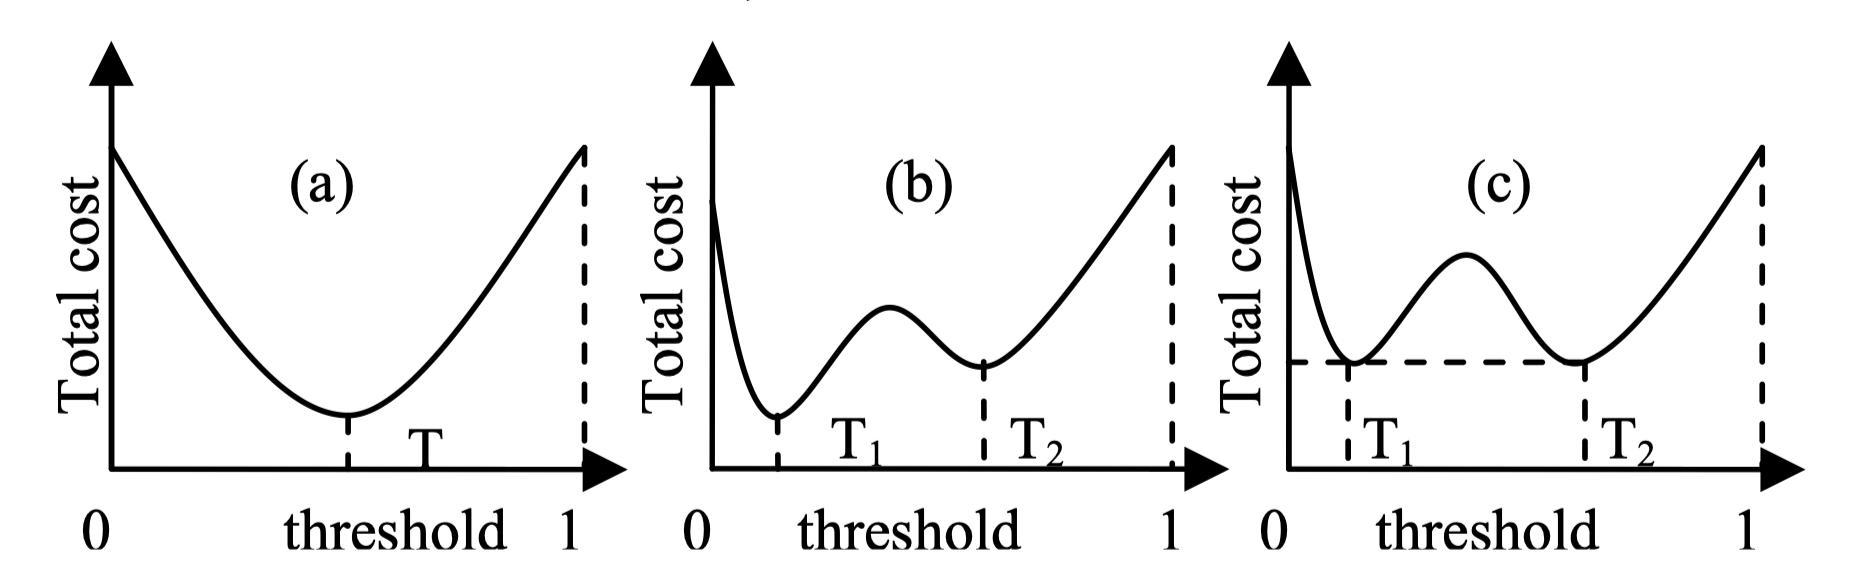
\includegraphics[width=0.95\textwidth]{figure/threshold_adjusting.png}
        \end{figure}

        %\item The optimal threshold $T^{*}$ corresponds to the point with the smallest $M_C$.

        \item What if two equal local minima? We prefer the one with wider span %(e.g. $T_2$ in the 3rd subfigure). Because it is less sensitive to small changes in $T$.

        \item Do this on validation data / over cross-val to avoid overfitting!
    \end{itemize}
\end{frame}

\begin{frame}{Empirical Thresholding: binary case}
    \begin{itemize}
        \item Example: German Credit task
        \footnotesize{
        \begin{center}
                            \begin{tabular}{cc|cc}
        			& &\multicolumn{2}{c}{True class} \\
        			& & $y=$ good & $y=$ bad  \\
        			\hline
        			\multirow{2}{*}{\parbox{0.3cm}{Pred.  class}} & $\hat y$ = good & 0 & 3 \\
        			& $\hat y$ = bad & 1 & 0\\
                \end{tabular}
        \end{center}
        }
        \item Theoretical: $C(good,bad)/(C(bad,good)+C(good,bad))=3/4=c^{*}$ 

        \item Empirical version with 3-CV: For XGBoost, empirical minimum deviates substantially from theoretical version

                \begin{figure}[h]
            \centering
            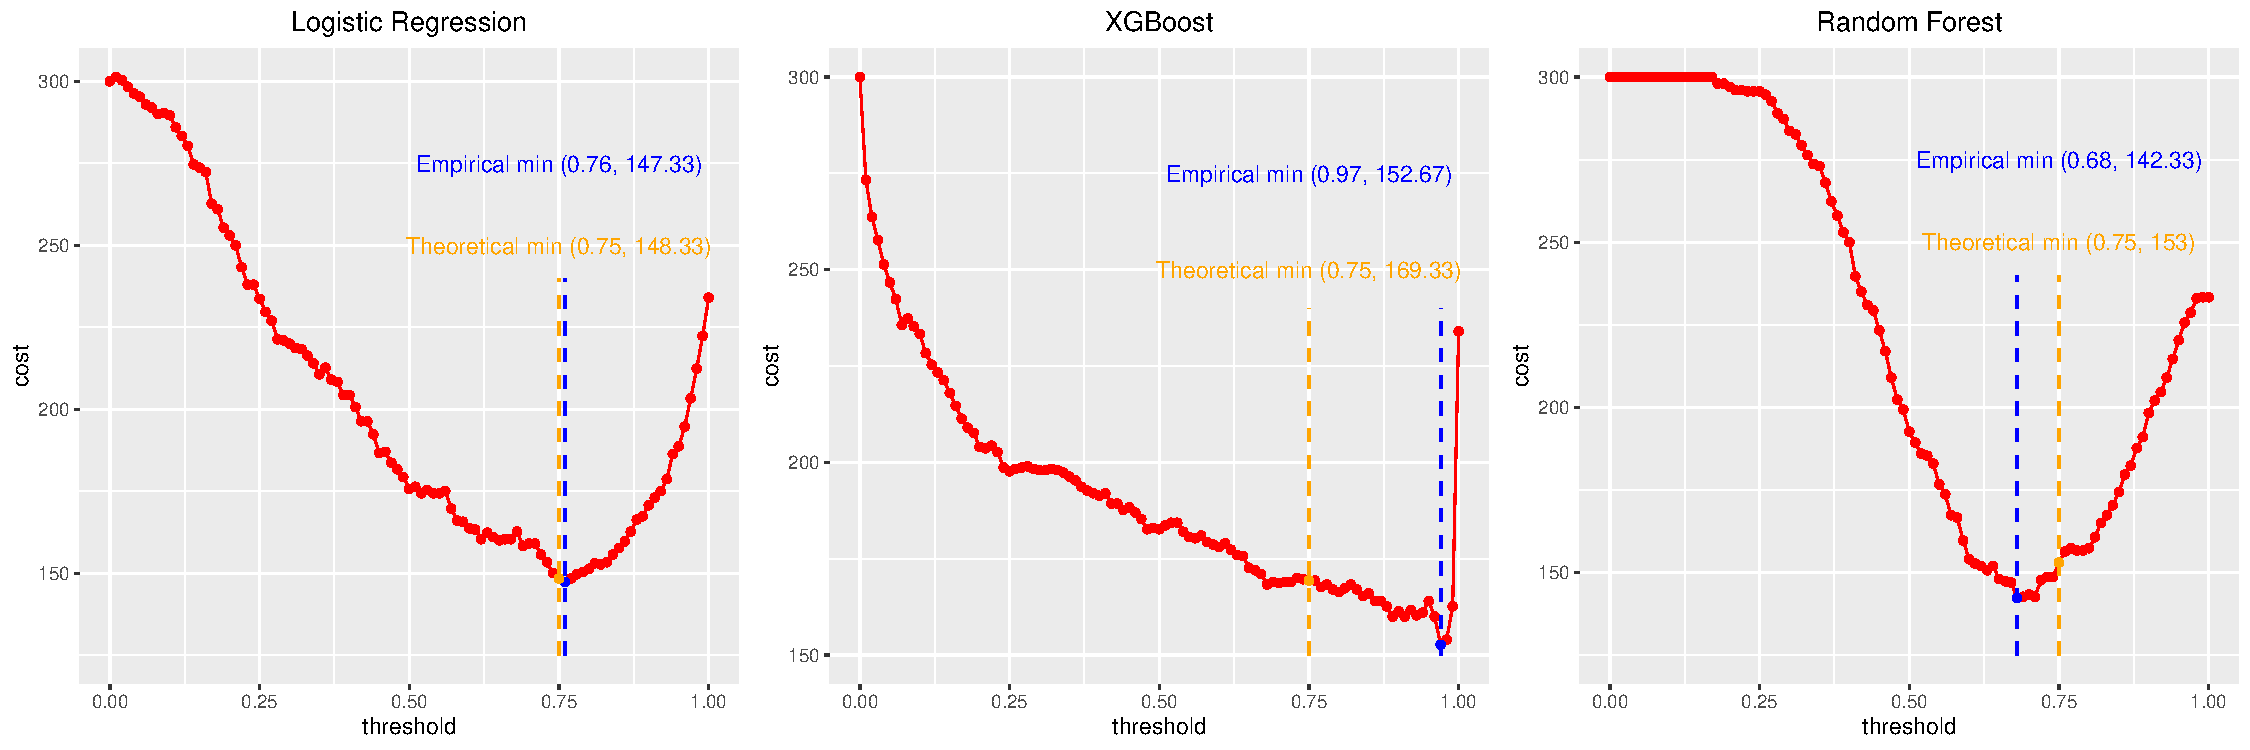
\includegraphics[width=0.95\textwidth]{figure_man/threshold_plots.pdf}
        \end{figure}

    \end{itemize}
\end{frame}


\begin{frame}{Empirical Thresholding: Multiclass}
    \begin{itemize}
 %        \item It is also possible to perform threshold adjusting in multi-class classifcation.
        
  %      \item Here, we present a simple approach for classifiers that output scores $\pi(\xv) = (\pi(\xv)_1,\ldots,\pi(\xv)_g)^\top$ in multi-class classification:
        
            \item In the standard setting, we predict class $h(\xv) = \argmaxlim_{k} \pikx$.
            
            \item Let's use $g$ thresholds $c_k$ now 
            
            \item Re-scale scores $ \mathbf{s} = (\frac{\pi(\xv)_1}{c_1},\ldots, \frac{\pi(\xv)_g}{ c_g})^\top$, 
            \item Predict class $\argmaxlim_k \pikx $.

            \item Compute empirical costs over cross-validation

            \item Optimize over $g$ (actually: $g-1$) dimensional threshold vector $(c_1, \ldots, c_g)^T$ to produce minimal costs

    \end{itemize}
\end{frame}

%\begin{frame}{MetaCost: Overview}
%
%        \begin{itemize}
%            \item Model-agnostic wrapper technique                      
%            \item General idea: 
%                \begin{enumerate}
%                \small
%                    \item Relabel train obs with their low expected cost classes
%                   
%                    \item Apply classifier to relabeled data
%                \end{enumerate} 
%                \item Example German Credit task:
%                                \begin{figure}[h]
%            \centering
%            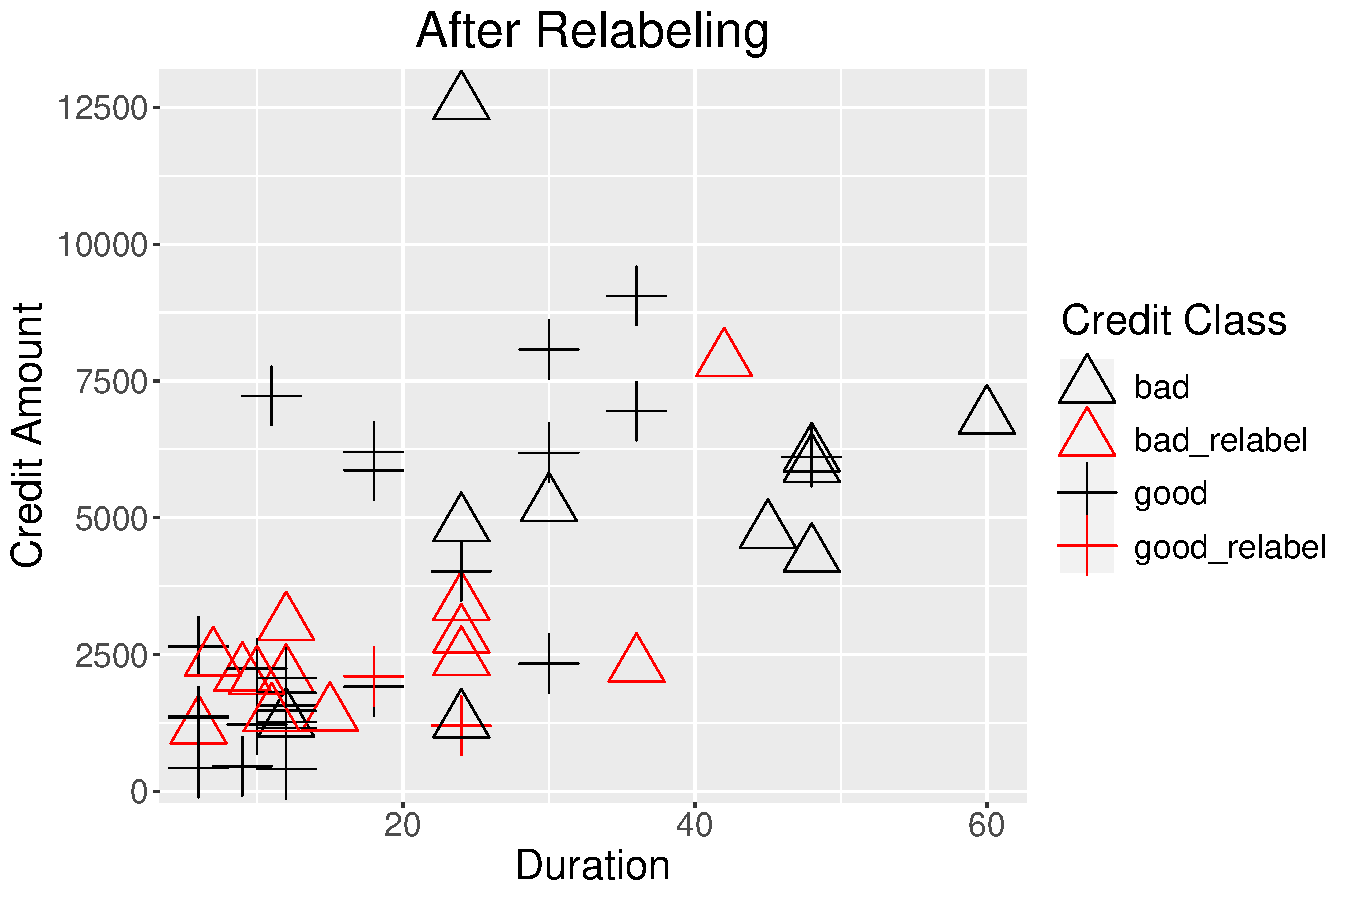
\includegraphics[width=0.5\textwidth]{figure_man/relabeling_viz.pdf}
%        \end{figure}
%                \item Relabeled instances colored red\
%                \item Relabeling from good to bad more common because of costs
%        \end{itemize}
%
%\end{frame}


%\begin{frame}{MetaCost: Algorithm}
%	
%		
%% 	The procedure of MetaCost is divided into three phases:
%			%			
%		% \begin{minipage}{0.59\textwidth} 
%		% 		\begin{itemize}
%		% 			\item \textcolor{teal}{Bagging --- Train $B$ times on bootstrapped data}
%  %    				\item \textcolor{blue}{Relabel --- Predict $\xi$ with classifiers that had it OOB and average}
%
%  %                       \item \textcolor{blue}{ Relabel --- Get new class by MECP}
%		% 			\item \textcolor{orange}{Cost-sens ---  Train on relabeled data}
%		% 		\end{itemize}
%		
%		% \end{minipage}
%			\begin{algorithmic}
%				
%				\scriptsize
%
%				\State \textbf{Input:} 
%				$\D = \{(\xi,\yi)\}_{i=1}^n$ training data, $B$ number of bagging iterations,
%				$\pix$ probabilistic classifier,
%				$\mathbf{C}$ cost matrix, empty dataset $\tilde D = \emptyset$ \\
%				 \textcolor{teal}{\# Bagging: Classifier is trained on different bootstrap samples.
%\For{$b=1,\ldots,B$}
%    \State $\D_b \leftarrow $ Bootstrap version of $\D$
%    \State $\pi_b \leftarrow $ train classifier on $\D_b$ 
%\EndFor 
%\\
%\textcolor{blue}{\# Relabeling: Find classifiers for which $\xi$ is OOB and compute $\pi_b$ by averaging over predictions.
%Determine new label $\tilde y^{(i)}$ w.r.t. to the cost minimal class.
%\For{$i=1,\ldots,n$}
% 	 \State $\tilde M \leftarrow \bigcup_{m: \xi \notin \D_m} \{m\}$ 
%\EndFor
%% \For{$i=1, \ldots n$}
%    \For{$j=1,\ldots,g$} 
%        \State $\pi_j(\xi)  \leftarrow \frac{1}{|\tilde M| } \sum_{m \in \tilde M}   \pi_j(\xi~|~ f_m)$ for each $i$ 
%    \EndFor
%% \EndFor
%\For{$i=1,\ldots,n$}
%\State $\tilde y^{(i)} \leftarrow \argmin_{k} \sum_{j=1}^g \pi_j(\xi) C(k,j) $
%\State $\tilde D \leftarrow \tilde D \cup \{(\xi,\tilde y^{(i)})\} $
%\EndFor}}  
%\\
%\textcolor{orange}{\# Cost Sensitivity: Train on relabeled data.\\
%$f_{meta} \leftarrow$ train $f$ on $\tilde D$}
%\end{algorithmic}
%
%\end{frame}

%%%
% reference: https://www.csie.ntu.edu.tw/~htlin/talk/doc/csovo.acml14.handout.pdf

\begin{frame}{Binary Instance-specific cost Learning}
    \begin{itemize}
        \item Assumes instance-specific costs for every observation:  $\D^{(n)} = \{(\xi, \cv^{(i)})\}_{i=1}^n$, where $(\xi, \cv^{(i)}) \in \mathbb{R}^p \times \mathbb{R}^2$.

        \item Define ``true class'' as cost minimal class
        
        \item Define observation weights: $|\cv^{(i)}[1] - \cv^{(i)}[0]|$
        % Consider four instances, where $\cv^{(i)}[0]$ and $\cv^{(i)}[1]$ denote the instance-wise cost of classifying an example as 0 or 1 respectively, $\yi$ the true label and 

        \begin{center}
            \begin{tabular}{cc|cccc}\
        			& & $\cv^{(i)}[0]$ & $\cv^{(i)}[1]$ & $\yi$ & $w^{(i)}$ \\
        			\hline & $\xv^{(1)}$ & 1 & 1 & 0 & 0\\
        			& $\xv^{(2)}$ & 1 & 2 & 0 & 1\\
        			& $\xv^{(3)}$ & 7 & 3 & 1 & 4\\
            \end{tabular}
        \end{center}

        \item Now solve weighted ERM:
        \begin{equation*}
            \mathcal{R}_{emp}(\boldsymbol{\theta}) = \sum_{i=1}^{n}w^{(i)} \Lxyit
        \end{equation*}
        
        \item NB: Instances with equal costs are effectively ignored.
        \end{itemize}
            
\end{frame}

\begin{frame}{Multiclass Costs}
    \begin{itemize}

        \item Consider $g > 2$. Vanilla CSL is special case of instance specific,\\use $\cv^{(i)}$ same for all $\xi$ of the same class
        %straightforward to see that class-specific cost-sensitive learning is a special case of instance-specific cost learning: 
        
        %\item Now consider a multiclass label space $\mathcal{Y}=\{1,2,3\}$. For class-specific cost sensitive learning, we may define the following cost matrix: 
        %\end{center}
        \vspace{5pt}
        
        \item For two $\xi$ with $y=2$ and $y = 3$: %instances of class 2 and 3 respectively, we have that
                \vspace{5pt}

                \begin{center}
                            \begin{tabular}{cc|cccc}\
        			& & $\cv^{(i)}[1]$ & $\cv^{(i)}[2]$ & $\cv^{(i)}[3]$ & $\yi$ \\
        			\hline & $\xv^{(1)}$ & \textcolor{blue}{1} & \textcolor{blue}{0} & \textcolor{blue}{1} & \textcolor{blue}{2}\\
        			& $\xv^{(2)}$ & \textcolor{green}{3} & \textcolor{green}{1} & \textcolor{green}{0} & \textcolor{green}{3}\\
                        & $\xv^{(3)}$ & \textcolor{blue}{1} & \textcolor{blue}{0} & \textcolor{blue}{1} & \textcolor{blue}{2}\\
                \end{tabular}
        \end{center}

        \item Set $\cv^{(i)}[\yi] = 0$, i.e. zero-cost for correct prediction.
        \vspace{5pt}
        
   %     \item Is the multiclass case restricted to class-specific cost sensitive learning? Of course not! Binary instance-specific cost learning can easily be generalized to the multiclass case. 
            
    \end{itemize}
\end{frame}

\begin{frame}{CSOVO}
    

    \begin{itemize}
        \item Let $\D^{(n)} = \{(\xi, \cv^{(i)})\}_{i=1}^n$, $(\xi, \cv^{(i)}) \in \mathbb{R}^p \times \mathbb{R}^g$.  
        \item Example:
       % Consider instance-specific costs for three observations of the form $(\xi, \yi, \cv^{(i)})$, with some label space $\mathcal{Y}=\{1, 2, \ldots, g\}$:

        \begin{center}
            \begin{tabular}{cc|ccc}\
        	& & $\cv^{(i)}[1]$ & $\cv^{(i)}[2]$ & $\cv^{(i)}[3]$  \\
        	\hline & $\xv^{(1)}$ & 0 & 2 & 3\\
        	& $\xv^{(2)}$ & 1 & 0 & 1\\
                 & $\xv^{(3)}$ & 2 & 0 & 3\\
            \end{tabular}
        \end{center}
        
        %\item Now: How to perform cost-sensitive learning when $g > 2$?
        
        \item Idea: Reduction principle to binary case (weighted fit) by one-versus-one (OVO). 
        %we have learnt cost-sensitive learning for the binary case. $\leadsto$ Convert the problem to 
        
        
        \item For class $j$ vs. $k$:
        %, consider two problems:
        \begin{itemize}
            \item How to deal with the label $\yi$? $\yi$ can be neither $j$ nor $k$.
            \vspace{5pt}
            
            \item How to deal with the costs $\cv^{(i)}[j]$ and $\cv^{(i)}[k]$?
            
        \end{itemize}
            
    \end{itemize}

\end{frame}


\begin{frame}{CSOVO}
    \begin{itemize}
        \item When training a binary classifier $f^{(j, k)}$ for class $j$ vs. $k$,
        \begin{itemize}
            \item Choose cost min class from pair $\argmin_{l \in \{j, k\}} \cv^{(i)}[l]$ as ground truth 
            
            \item Sample weight is simply diff between the 2 costs      $|\cv^{(i)}[j] - \cv^{(i)}[k]|$

            %\item After cost transformation, the misclassification costs across classes are equal to 1. $\leadsto$ Sample-wise weighted binary classification problem.
        \end{itemize}
        
        \item Example continued:
\begin{center}
    \footnotesize
                            \begin{tabular}{cc|ccc|ccc}\
        			& & $\cv^{(i)}[1]$ & $\cv^{(i)}[2]$ & $\cv^{(i)}[3]$ & $\cv^{(i)}[1 \ \text{vs} \ 2]$ & $\tilde{y}^{( i)}[1 \ \text{vs} \ 2]$ & $w^{(i)}[1 \ \text{vs} \ 2]$\\
        			\hline & $\xv^{(1)}$ & 0 & 2 & 3 & 0/2 & 1 & 2\\
        			& $\xv^{(2)}$ & 1 & 0 & 1 & 1/0 & 2 & 1 \\
                 	& $\xv^{(3)}$ & 2 & 0 & 3 & 2/0 & 2 & 2\\
                \end{tabular}

                \begin{tabular}{cc|ccc|ccc}
        			& & $\cv^{(i)}[1]$ & $\cv^{(i)}[2]$ & $\cv^{(i)}[3]$ & $\cv^{(i)}[2 \ \text{vs} \ 3]$ & $\tilde{y}^{( i)}[2 \ \text{vs} \ 3]$ & $w^{(i)}[2 \ \text{vs} \ 3]$\\
        			\hline & $\xv^{(1)}$ & 0 & 2 & 3 & 2/3 & 2 & 1\\
        			& $\xv^{(2)}$ & 1 & 0 & 1 & 0/1 & 2 & 1\\
                 	& $\xv^{(3)}$ & 2 & 0 & 3 & 0/3 & 2 & 3\\
                \end{tabular}
\end{center}

    \end{itemize}
\end{frame}


\begin{frame}{CSOVO}
    \begin{itemize}
    \item Example continued
    \begin{center}  
        \footnotesize{
            \begin{tabular}{cc|ccc|ccc}
                & & $\cv^{(i)}[1]$ & $\cv^{(i)}[2]$ & $\cv^{(i)}[3]$ & $\cv^{(i)}[1 \ \text{vs} \ 3]$ & $\tilde{y}^{( i)}[1 \ \text{vs} \ 3]$ & $w^{(i)}[1 \ \text{vs} \ 3]$\\
                \hline & $\xv^{(1)}$ & 0 & 2 & 3 & 0/3 & 1 & 3\\
                & $\xv^{(2)}$ & 1 & 0 & 1 & -/- & - & 0 \\
                & $\xv^{(3)}$ & 2 & 0 & 3 & 2/3 & 1 & 1\\
            \end{tabular}
        }
    \end{center}

    \item Wrap everything up:
    \begin{enumerate}
        \item For class $j$ vs. $k$, transform all $(\xi, \cv^{(i)})$ to $(\xi, \argmin_{l \in \{j, k\}} \cv^{(i)}[l])$ with sample-wise weight $|\cv^{(i)}[j] - \cv^{(i)}[k]|$.
        
        \item Train a weighted binary classifier $f^{(j, k)}$ using the above
        
        \item Repeat step 1 and 2 for different $(j, k)$.
        
        \item Predict using the votes from all $f^{(j, k)}$.
    \end{enumerate}

    \item Theoretical guarantee:\\ 
    test costs of final classifier $\leq 2\sum_{j < k}$ test cost of $f^{(j, k)}$. 
    \end{itemize}
\end{frame}


%\begin{frame}{MetaCost: Example}
%	%	
%	\small{
%		\begin{itemize}
%			%		
%			\item We compare C4.5 (decision tree) with MetaCost using C4.5 for the \href{http://staffwww.itn.liu.se/~aidvi/courses/06/dm/
%				labs/heart-c.arff}{heart data set}  in \href{ http://www.cs.waikato.ac.nz/ml/weka/}{Weka}. 
%			%		
%			\item The cost matrix $\mathbf{C}$ is 
%			
%			\begin{center}
%				\begin{tabular}{cc|cc}
%					& &\multicolumn{2}{c}{True class} \\
%					& & $y=1$ & $y=-1$  \\
%					\hline
%					\multirow{2}{*}{\parbox{0.3cm}{Pred.  class}}& $\hat y$ = 1     & $0$                & $ 1 $\\
%					& $\hat y$ = -1 & $ 4 $              &  $0$   \\
%				\end{tabular}
%			\end{center}
%		
%			\item The resulting confusion matrices are 
%			
%						
%			\begin{center}
%				\begin{tabular}{cc|cc}
%					& &\multicolumn{2}{c}{True class} \\
%					& MetaCost & $y=1$ & $y=-1$  \\
%					\hline
%					\multirow{2}{*}{\parbox{0.3cm}{Pred.  class}}& $\hat y$ = 1     & $104$                & $ 21 $\\
%					& $\hat y$ = -1 & $ 61 $              &  $117$   \\
%				\end{tabular}
%							\begin{tabular}{cc|cc}
%				& &\multicolumn{2}{c}{True class} \\
%				& C4.5 & $y=1$ & $y=-1$  \\
%				\hline
%				\multirow{2}{*}{\parbox{0.3cm}{Pred.  class}}& $\hat y$ = 1     & $138$                & $ 40 $\\
%				& $\hat y$ = -1 & $ 27$              &  $98$   \\
%			\end{tabular}
%			\end{center}
%		
%		
%			%		
%			\item The total cost of MetaCost is 145, while C4.5 has total costs of 187. However, MetaCost has $0.729$ correct classifications and C4.5 has $0.779.$ 
%			
%			%		
%		\end{itemize}
%		%
%	}
%	%	
%\end{frame}



%\begin{frame}{Cost-Sensitive Decision Trees}
%	%	
%	\small{
%		\begin{itemize}
%			%		
%			\item 
%			%		
%		\end{itemize}
%		%
%	}
%	%	
%\end{frame}


%
% https://github.com/slds-lmu/lecture_advml/blob/main/slides/imbalanced-learning/slides-imbalanced-learning-sampling-methods-1.tex
\section{Under- and Oversampling}

\begin{frame}{Sampling Methods: Overview}
    \small{
		\begin{itemize}
			\item Balance training data distribution to perform better on minority classes.
			
			\item Independent of classifier $\leadsto$ very flexible and general.
   
			\item Three groups: 
		
			\begin{minipage}{0.59\textwidth}
				\begin{itemize} 
                    % Need this \small, otherwise the fontsize will be the default size.
                    \small
                    
					\item Undersampling --- Removing instances of majority class(es).
			
					\item Oversampling --- Adding/Creating new instances of minority class(es).  (Slower, but usually works better.)

                    %\item Oversampling is slower, but usually works better.

					\item Hybrid --- Combining both methods.
			
				\end{itemize}
			\end{minipage}
            \hfill
			\begin{minipage}{0.3\textwidth}
					\begin{figure}[c]
					\centering
                    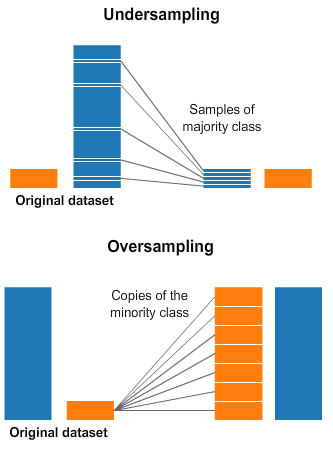
\includegraphics[width=\textwidth]{figure/under_oversampling.png}
				\end{figure}
			\end{minipage}
		\end{itemize}
	}
\end{frame}
	
\begin{frame}{Random Undersampling/Oversampling}

    \begin{itemize}
        \item Random oversampling (ROS):
        \begin{itemize}
            \item Randomly \textbf{replicate} \textbf{minority} instances.% until a desired imbalance ratio.
            \item Prone to overfitting due to multiple tied instances.
        \end{itemize}

        \item Random undersampling (RUS):
        \begin{itemize}
            \item Randomly \textbf{eliminate} \textbf{majority} instances. % until a desired imbalance ratio.
            \item Might remove informative instances and destroy important concepts in data.
        \end{itemize}

        \item Better: Introduce heuristics in removal process (RUS) and do not create exact copies (ROS).
    
        \end{itemize}	

\end{frame}
	
\begin{frame}{Undersampling: Tomek Links}
    \small{

        \begin{itemize}            
            \item Remove ``noisy borderline'' examples (very close observations of different classes) of majority class(es).
%            \item Noisy borderline examples are ``very close'' observations of different classes.
            % \begin{itemize}
            %     % Need this \footnotesize to maintain fontsize
            %     \footnotesize
            %     \item From different classes.
            %     \item ``Very close'' to each other.
            % \end{itemize} 
            \item Let $E^{(i)} = (\xi,\yi)$ and $E^{(j)} = (\xv^{(j)},y^{(j)})$ be two data points in $\D$. % with $\yi\neq y^{(j)}.$
        \end{itemize}
        \begin{columns}
            \begin{column}{0.7\textwidth}	
        
                \begin{itemize}

                    %\vspace{10pt}
                    
                    \item A pair $(E^{(i)},E^{(j)})$ is called \emph{Tomek link} iff there is no other data point $E^{(k)} = (\xv^{(k)},y^{(k)})$ such that
        
                    \begin{itemize} 
                    \footnotesize
                
                       \item [] $d(\xv^{(i)}, \xv^{(k)}) < d(\xv^{(i)}, \xv^{(j)}) $ or
                       \item [] $d(\xv^{(j)}, \xv^{(k)}) < d(\xv^{(i)}, \xv^{(j)}) $ holds,
                    
                    \end{itemize}
        
                where $d$ is some distance on $\Xspace.$
                \item $\yi \neq \yi[j]$% E^{(i)}$ and $E^{(j)}$ have different $y$'s 
                $\leadsto$ noisy borderline examples.

                \item Remove majority instance in each data pair in a Tomek link where $\yi \neq \yi[j]$.

                %\item No random sampling here, but it can be combined with RUS.
                
                \end{itemize}		
            \end{column}
        
            \begin{column}{0.3\textwidth}
                \begin{figure}
                    \centering
                    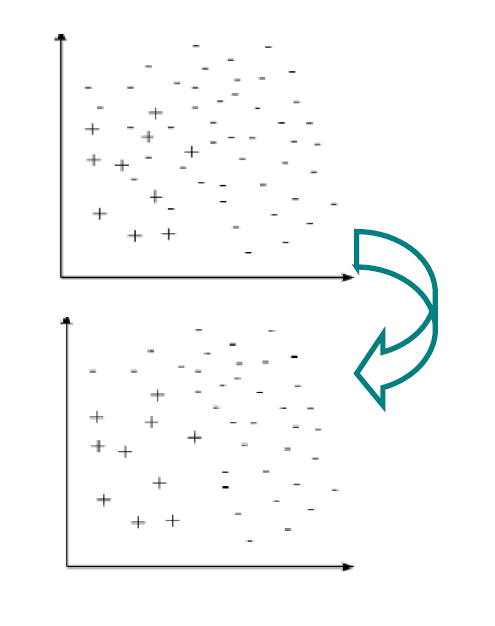
\includegraphics[width=0.85\textwidth]{figure/tomek_link_plot.png}	
                    \tiny
                    \\ Franciso Herrera (2013), Imbalanced Classification: Common
                    Approaches and Open Problems (\href{https://sci2s.ugr.es/sites/default/files/files/TutorialsAndPlenaryTalks/SSTiC-Trends in-Classification-Imbalanced-data-sets.pdf}{\underline{URL}}).
                \end{figure}
            \end{column}
        \end{columns}
   }
\end{frame}

%  \begin{frame}{Undersampling: Tomek Links}

%     \begin{columns}
%         \begin{column}{0.59\textwidth}
%             \begin{itemize} 
                
%                  \item A pair $(E^{(i)},E^{(j)})$ is called \emph{Tomek link} iff there is no other data point $E^{(k)} = (\xv^{(k)},y^{(k)})$ such that $d(\xv^{(i)}, \xv^{(k)}) < d(\xv^{(i)}, \xv^{(j)}) $ or $d(\xv^{(j)}, \xv^{(k)}) < d(\xv^{(i)}, \xv^{(j)}) $ holds.
                
%                 \item $E^{(i)}$ and $E^{(j)}$ have different $y$'s $\leadsto$ a bordeline case.

%                 \item Remove majority instance in each data pair in a Tomek link.

%                 \item No random sampling here, but can be combined with RUS.

            
%             \end{itemize}
%         \end{column}

%         \begin{column}{0.4\textwidth}
%             \begin{figure}
%                 \centering
%                 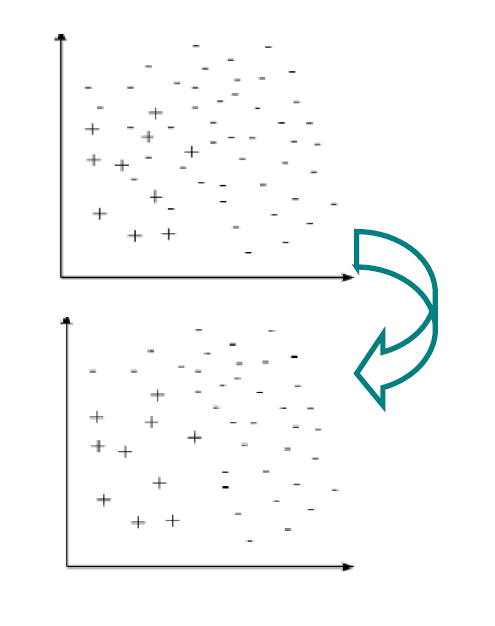
\includegraphics[width=0.85\textwidth]{figure/tomek_link_plot.png}	\tiny
%                 \\ Franciso Herrera (2013), Imbalanced Classification: Common
%                 Approaches and Open Problems (\href{https://sci2s.ugr.es/sites/default/files/files/TutorialsAndPlenaryTalks/SSTiC-Trends in-Classification-Imbalanced-data-sets.pdf}{\underline{URL}}).
%             \end{figure}
%         \end{column}
%     \end{columns}

% \end{frame}
	
	
% \begin{frame}{Undersampling: Condensed Nearest Neighbor (CNN)}
	
%     \begin{itemize}
    
%         \item Remove majority instances far away from decision boundary. 
%         \item Construct a \textbf{consistent} subset $\tilde{\D}$ of $\D$. % in terms of the 1-NN classifier. 

%         \item A subset $\tilde{\D}$ of $\D$ is called consistent if using a 1-NN classifier on $\tilde{\D}$ classifies each instance in $\D$ correctly.

% %     \end{itemize}	

% % \end{frame}

% % \begin{frame}{Undersampling: Condensed Nearest Neighbor (CNN)}
% %     \begin{itemize}
%         \item Create a consistent subset:
        
%         \begin{enumerate}
    
%             \item Initialize $\tilde{\D}$ by selecting \textbf{all minority} instances and randomly picking \textbf{one majority} instance.
    
%             \item Classify each instance in $\D$ with 1-NN classifier based on $\tilde{\D}.$
        
%             \item Remove all misclassified instances from $\D$.
            
%         \end{enumerate}	
    
%     \end{itemize}
    
    
% \end{frame}
	
\begin{frame}{Undersampling: Other Approaches}

    \begin{itemize}

        \item Neighborhood cleaning rule (NCL):
    
        \begin{enumerate}
            
            \item Find 3 nearest neighbors for each $(\xi,\yi)$ in $\D.$
        
            \item If $\yi$ is majority class \emph{and} 3-NN classifies it as minority $\leadsto$ Remove $(\xi,\yi)$ from $\D$.
        
            \item If $\yi$ is minority class \emph{and} 3-NN classifies it as majority $\leadsto$ Remove 3 nearest neighbors from $\D$.
        
        \end{enumerate} 

    \item Condensed Nearest Neighbor (CNN): Construct a \textbf{minimally consistent} subset $\tilde{\D}$ of $\D$.
        \item One-sided selection (OSS): Tomek link + CNN

        \item CNN + Tomek link: to reduce computation of finding Tomek links $\leadsto$ first use CNN and then remove the Tomek links.
    
        \item Clustering approaches: Class Purity Maximization (CPM) and Undersampling based on Clustering (SBC).

    \end{itemize}

\end{frame}
	
% \begin{frame}{Oversampling: SMOTE}

%     \begin{itemize}	
%         \item The Synthetic Minority Oversampling Technique (SMOTE) operates by creating \textbf{new synthetic examples} of minority class.

%         \item Interpolate between neighboring minority examples.

%         \item Examples are created in $\Xspace$ rather than in $\Xspace\times\Yspace.$

%         \item Algorithm: For each minority instance: 

%         \begin{itemize} 

%             \item Find $k$ nearest minority neighbors.
    
%             \item Randomly select $j$ of these neighbors.
    
%             \item Randomly generate new instances along the lines connecting the minority instance and its $j$ neighbors.
    
%         \end{itemize}

%     \end{itemize}

%     \begin{figure}
%         \centering
%         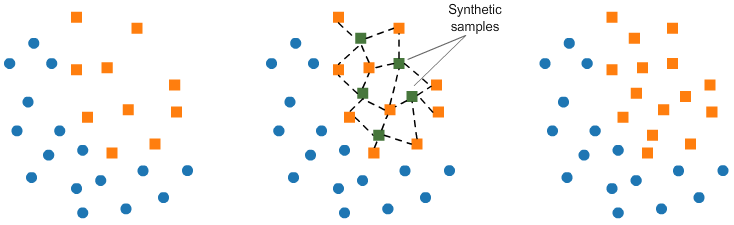
\includegraphics[width=0.8\textwidth]{figure/SMOTE.png} 
%     \end{figure}

% \end{frame}

% https://github.com/slds-lmu/lecture_advml/blob/main/slides/imbalanced-learning/slides-imbalanced-learning-sampling-methods-2.tex
\section{SMOTE}

% \begin{frame}{Sampling Methods: Overview}
%     \begin{itemize}

%         \item Balance training data distribution to perform better on minority classes.
        
%         \item Independent of classifier $\leadsto$ very flexible and general.

%         \item Three groups: 
    
%         \begin{minipage}{0.5\textwidth}
    
%             \begin{itemize} 
                
%                 \item Undersampling --- Removing majority instances.
        
%                 \item Oversampling --- Adding/Creating new minority instances.

%                 \item Oversampling is slower than undersampling but usually works better.

%                 \item Hybrid approaches --- Combining undersampling and oversampling.
        
%             \end{itemize}
    
%         \end{minipage}
%         \begin{minipage}{0.4\textwidth}
%                 \begin{figure}
%                 \centering
%                 \scalebox{0.8}{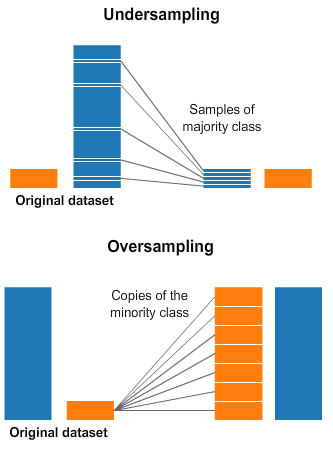
\includegraphics{figure/under_oversampling.png}}
%             \end{figure}
%         \end{minipage}

%     \end{itemize}
    
% \end{frame}


\begin{frame}{Oversampling: SMOTE}
    \begin{itemize}
        %			
        \item SMOTE creates \textbf{synthetic instances} of minority class.

        \item Interpolate between neighboring minority instances.

        \item Instances are created in $\Xspace$ rather than in $\Xspace\times\Yspace.$

        \item Algorithm: For each minority class instance: 

        \begin{itemize} 

            \item Find its $k$ nearest minority neighbors.
    
            \item Randomly select one of these neighbors.
    
            \item Randomly generate new instances along the lines connecting the minority example and its selected neighbor.
    
        \end{itemize}
    \end{itemize}
    
    \begin{figure}
        \centering
        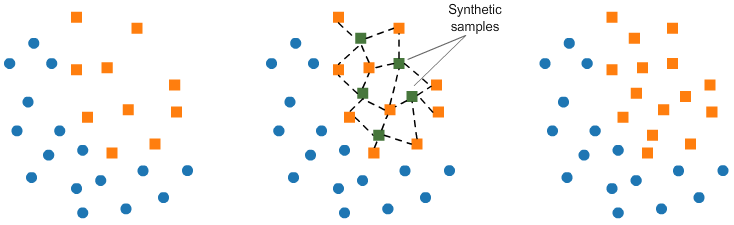
\includegraphics[width=0.8\textwidth]{figure/SMOTE.png} 
    \end{figure}


\end{frame}

\begin{frame}{SMOTE: Generating new examples}
    
    \begin{itemize}

        \item Let $\xi$ be the feature of the minority instance and let $\xv^{(j)}$ be its nearest neighbor. The line connecting the two instances is
        $$		(1-\lambda) \xi + \lambda\xv^{(j)} = \xi + \lambda(\xv^{(j)} - \xi)	$$
        where $\lambda \in [0,1].$		
        
        \item By sampling a $\lambda \in [0,1],$ say $\tilde{\lambda},$ we create a new instance		
        $$   \tilde{\xv}^{(i)} =  \xi + \tilde{\lambda}(\xv^{(j)} - \xi)	 $$

    \end{itemize}		
        
        Example: Let $\xi = (1,2)^\top$ and $\xv^{(j)} = (3,1)^\top.$ Assume $\tilde{\lambda} \approx 0.25.$
        %
    \begin{figure}
        \centering
        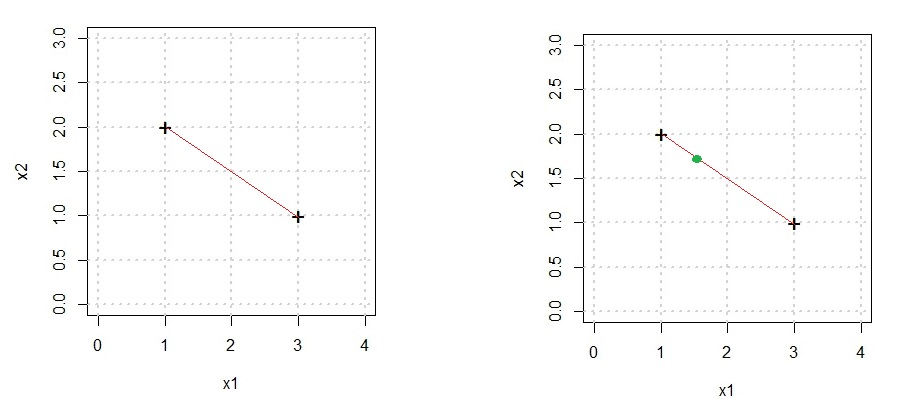
\includegraphics[width=0.8\linewidth]{figure_man/coordinate_system}
    \end{figure}

\end{frame}


\begin{frame}{SMOTE: Visualization}
    
    For an imbalanced data situation, take four instances of the minority class. Let $K=2$ be the number of nearest neighbors.		

        \begin{figure}
            \centering
            \foreach \x in{1,2,3,4,5,6,7,8,9,10} {
            \includegraphics<\x>[width=0.8\linewidth]{figure_man/smote_viz_\x.pdf}\par
            }
        \end{figure}
\end{frame}

\begin{frame}{SMOTE: Visualization continued}

    After 100 iterations of SMOTE for $K=2$ we get:		

    \begin{figure}
        \centering
        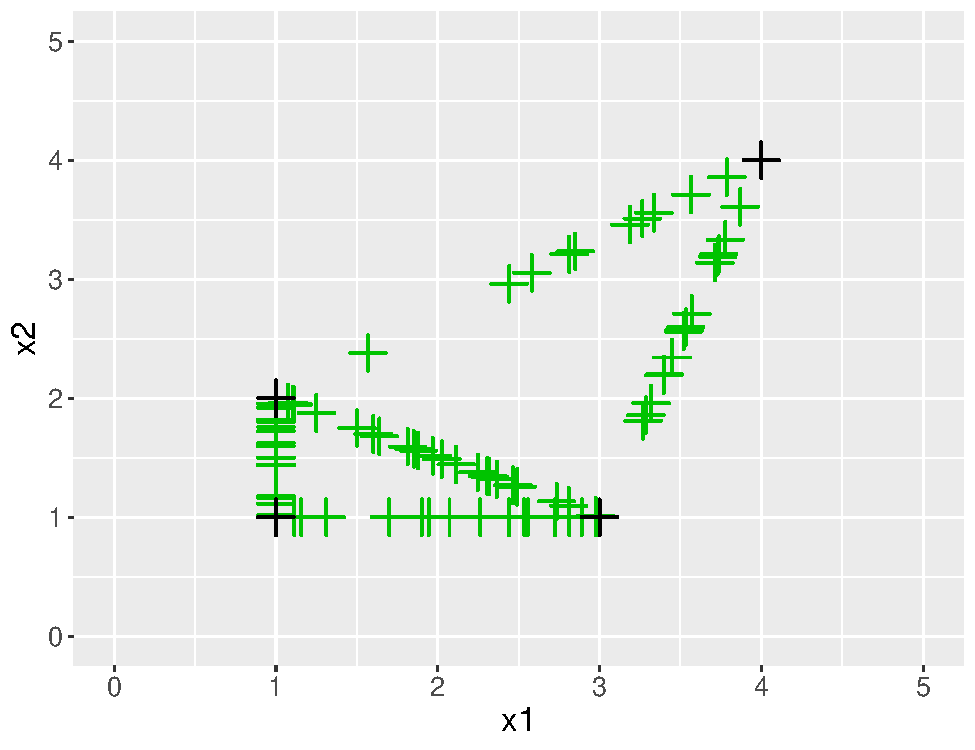
\includegraphics[width=0.8\linewidth]{figure_man/smote_viz_11.pdf}
    \end{figure}

\end{frame}

\begin{frame}{SMOTE: Visualization continued}	

    After 100 iterations of SMOTE for $K=3$ we get:		

    \begin{figure}
        \centering
        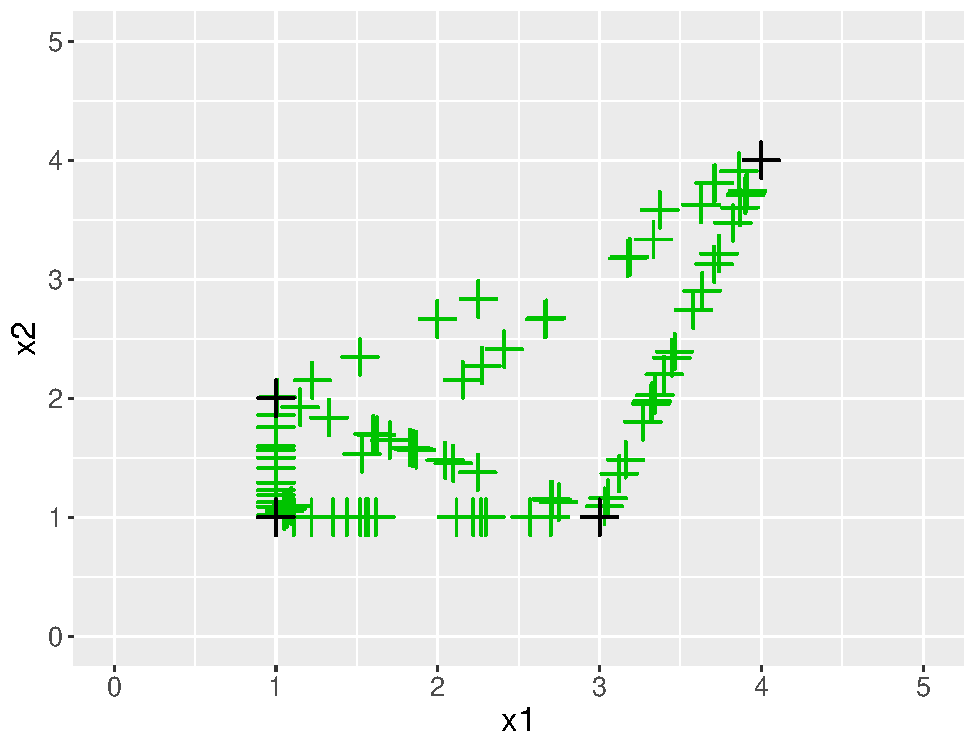
\includegraphics[width=0.8\linewidth]{figure_man/smote_viz_12.pdf}
    \end{figure}
	
\end{frame}
    
\begin{frame}{SMOTE: Example}
    
    \begin{itemize}
        \item Iris data set with 3 classes % $\Yspace=\{ \texttt{setosa},\texttt{versicolor},\texttt{virginica}  \}$, 
        and 50 instances per class.
        
        \item Make the data set ``imbalanced'': 
        \begin{itemize}
            \item relabel one class as positive
            \item relabel two other classes as negative
        \end{itemize}
    \end{itemize}		

    \begin{figure}
        \centering
        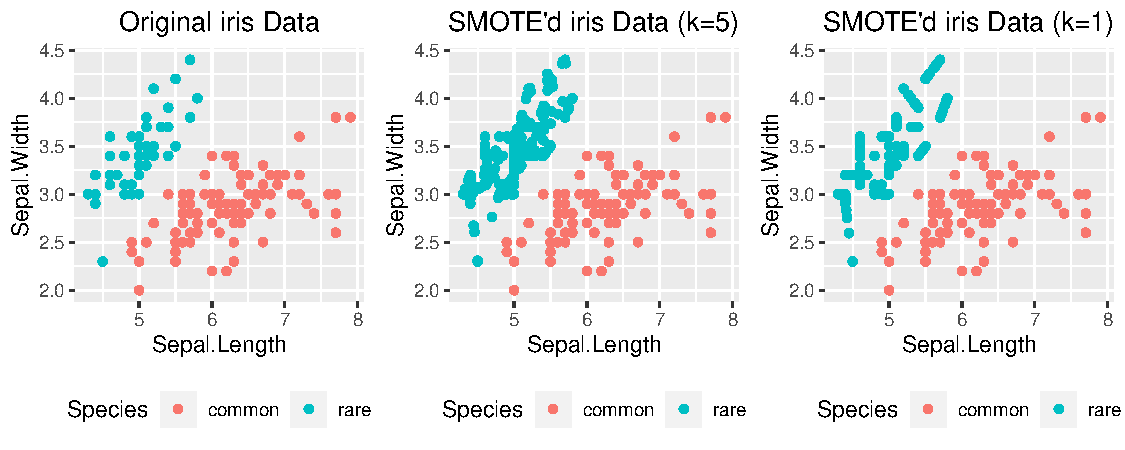
\includegraphics[width=0.9\linewidth]{figure_man/smoted_iris_data_ggplot.pdf}
    \end{figure}

SMOTE enriches minority class feature space.
	
\end{frame}


\begin{frame}{SMOTE: Dis-/Advantages}

    \begin{itemize}
    
        \item Generalize decision region for minority class instead of making it quite specific, such as by random oversampling. 
        
        \item Well-performed among the oversampling techniques and is the basis for many oversampling methods: Borderline-SMOTE, LN-SMOTE, $\ldots$ (over 90 extensions!)
    
        \item Prone to overgeneralizing as it pays no attention to majority class.

    \end{itemize}		

\end{frame}

\begin{frame}{Comparison of Sampling Techniques}

    \begin{itemize}
    
        \item Compare different sampling techniques on a binarized version of Optdigits dataset for optical recognition of handwritten digits.
    
        \item Use random forest with 100 trees, 5-fold cv, and $F_1$-Score. %The pos./neg. class-ratios are 0.11, 0.68, 0.68, and 0.79:
           \begin{center}
             \begin{tabular}{lrr}
             \toprule
             Sampling technique & Class ratio &F1-Score\\
             \midrule
             None & 0.11 &0.9239\\
             Undersampling & 0.68 & 0.9538\\
             Oversampling & 0.69& 0.9538\\
             SMOTE & 0.79 & 0.9576\\
             \bottomrule
             \end{tabular}    
            \end{center}
            
        \item Class ratios could be tuned (here done manually).
        \item Sampling techniques outperform base learner. 
        \item SMOTE leads sampling techniques, although by a small margin.

    \end{itemize}		

\end{frame}

\section{Conclusion}

\begin{frame}{When to counteract imbalanced data?}
\begin{itemize}
    \item Only counteract if your metric is impacted by imbalanced data
    \item How to counteract? Can you change to a metric that is not affected by imbalanced data?
    \item Check if treatment of imbalanced data has any adversarial effects \href{https://arxiv.org/abs/2404.19494}{\beamergotobutton{REF}}
    \item Try simple methods first, especially SMOTE is highly criticized \href{https://arxiv.org/abs/2201.08528}{\beamergotobutton{REF}}
    \item Use hyperparameter optimization to decide what method to use.
    \item Why not treat finding the trade-off between precision and recall as a multi-objective hyperparameter optimization problem?
\end{itemize}
    
\end{frame}

\endlecture
\end{document}